\documentclass{book}
\usepackage{graphicx}
\usepackage{html} %% from latex2html
%%\usepackage{times}
\begin{document}

\begin{titlepage}
\begin{center}


\includegraphics{ImgPrlg.png}

\vspace{0.7cm}

{\Huge PROLOG+CG version 2.0}

\vspace{1.5cm}

{\huge User's Manual}

\vspace{1.5cm}

{\Large By Dr. Adil KABBAJ\footnote{I.N.S.E.A, Rabat, Morocco. {\bf E-mail:} \texttt{akabbaj\{a-t\}insea\{d-ot\}ac\{do-t\}ma}}}

\bigskip

{\Large Modified by Ulrik Petersen\footnote{Aalborg University, Denmark. {\bf E-mail:} \texttt{ulrikp\{at\}users\{d-ot\}sourceforge\{do-t\}net}}}

\vspace{1.6cm}

2005-06-22

\vspace{1.6cm}

{\large {\bf Web:} \texttt{http://prologpluscg.sourceforge.net/}}

\end{center}
\end{titlepage}


\tableofcontents{}

\vspace{2cm}

\section*{Feedback}

Please report any bugs, problems or suggestions to Ulrik Petersen at:

\begin{center}
\texttt{ulrikp\{a-t\}user\{do-t\}sourceforge\{do-t\}net}
\end{center}

{\bf Please do not contact Prof. Kabbaj about Prolog+CG 2.0}.  Contact
Ulrik Petersen instead.

Please note that Prolog+CG version 2.0 is {\bf legacy code},
maintained by Ulrik Petersen.  A new and better version, version 3,
has been released as part of the Amine-platform:
\texttt{<http://amine-platform.sourceforge.net>}.

\newpage

\chapter{Basics}

\section{Introduction}\label{Sec:Introduction}

PROLOG (PROgramming in LOGic) is a programming language that has been
designed first (around 1972) for natural language processing and
theorem proving. It has been used, since that time in many fields of
Artificial Intelligence (AI).  Now, PROLOG is a standard programming
language in AI.

This manual is not about PROLOG, even if a quick introduction of
this language is given as the basic elements of PROLOG+CG are
introduced. Several books and documentation concerning PROLOG language
are available. This manual is about a descendant of PROLOG :
{\bf PROLOG+CG} which is {\bf {\it a conceptual and an
object-oriented extension of PROLOG}}. Indeed, to achieve
more expressive power, the PROLOG language has been extended, in the
past, in at least two directions :

\begin{itemize}

\item {\bf {\it Conceptual extension} :} a goal can be
represented by a term (a predicate) or by a complex structure, like
typed feature structure [1, 2, 3, 10, 18].

\item {\bf {\it Contextual extension} :} it is illustrated
first by object-based PROLOG [14, 16, 4, 5] where a Prolog program is
partitioned into objects (or worlds, theories, modules, bases, spaces
or other similar terms), each object contains a set of rules. A goal
is then resolved in the context of a specific object. Contextual
extension of PROLOG is illustrated also by object-oriented PROLOG [7,
15, 17] where inheritance between objects is considered.

\end{itemize}

{\it {\bf PROLOG+CG is a conceptual extension of PROLOG in the sense
that}} it integrates Conceptual Graphs (CG) at the basic
level. Conceptual Graph (CG) formalism (for background knowledge about
conceptual graphs, please see:
\verb+http://www.jfsowa.com/cg/index.htm+) is a synthesis of several
works on semantic networks. CG has been used in many fields of AI,
especially natural language processing and knowledge base systems. An
integration of CG to Prolog is very interesting. In the Conceptual
Graph community, some systems [6, 8, 9] incorporated a deductive
component that interprets a set of rules, all the goals of a rule are
represented by simple Conceptual Graphs (CG). However, these
components do not subsume PROLOG and were not presented as extensions
of PROLOG. For instance, no work has been done in the past to develop
a Prolog version that provides CG as a basic data structure, beside
term and list. PROLOG+CG fulfills this gap in the CG research (i.e., a
need for a CG based extension of Prolog) : CG can be used to represent
goals (beside terms) and can be used and manipulated as basic data
structures, with operations like maximal join, projection (or more
precisly subsumption), generalization and unification operations.

PROLOG+CG is a contextual extension of PROLOG in the sense that it
integrates notions like objects and inheritance.

Also, PROLOG+CG integrates JAVA : PROLOG+CG can be called from a Java
program and a Prolog+CG program can call Java classes.

The integration of {\bf Prolog}, {\bf object oriented programming},
the {\bf manipulation of CG} and {\bf Java} provides a powerful
development environment for the creation of knowledge-based
applications and their integration on the web. Java allows the
development of multi-platform applications as well as the capabilities
of object-oriented languages. Prolog provides the full power of a
logic programming language well suited for natural language
processing, inference and symbolic manipulations. CGs provide the
expressive power of an advanced knowledge representation language
(advanced semantic nets, type hierarchy, schemas, notion of context,
etc.).

PROLOG+CG is implemented in JAVA 2. A beta version 2.0 is available
through the site \verb+http://prologpluscg.sourceforge.net/+

Please note that Prolog+CG version 2 is {\it legacy code}, maintained
by Ulrik Petersen.  A new and better version is available as part of
the Amine platform.

\section{Prolog+CG and its installation}\label{Sec:EnvAndInstall}

The integrated environment of PROLOG+CG consists of a text editor, a
``compiler'', the debugger and the interpreter. The compiler performs
a syntactic analysis of the program and if the analysis is successful,
it generates an object file that contains an internal representation
of the program, in terms of Java structures (vector, hashtable,
etc.). Thereafter, the interpreter works on the object file.

At the interface level, the environment provides a split pane; the top
pane is used to create/open/edit a program while the bottom pane is
used as a console : the user asks a request and the system gives the
answer (Figure \ref{PrologPlusCGEnvironment}). During the compilation,
the console pane becomes a compiler pane where messages concerning
this task are written. If the compilation has been successfull, the
user has to click inside the pane to switch to the console pane.

The environment provides also a debug window (accessible from the
Build menu) and a window that shows the primitive operations of the
language (accessible from the Help menu).

Figure \ref{PrologPlusCGEnvironment} gives a snapshot of the PROLOG+CG
environment.

\begin{latexonly}

\begin{figure}
\begin{center}
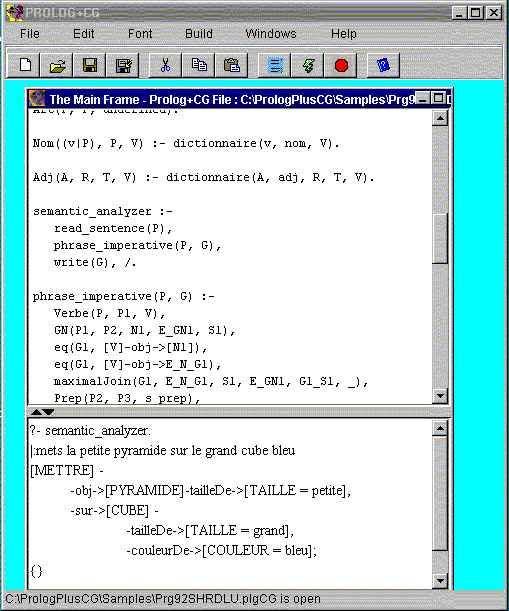
\includegraphics[scale=0.4]{snapshot1.png}
\end{center}
\caption{\label{PrologPlusCGEnvironment}PROLOG+CG Environment}
\end{figure}

\end{latexonly}

\begin{htmlonly}

\begin{figure}
\begin{center}
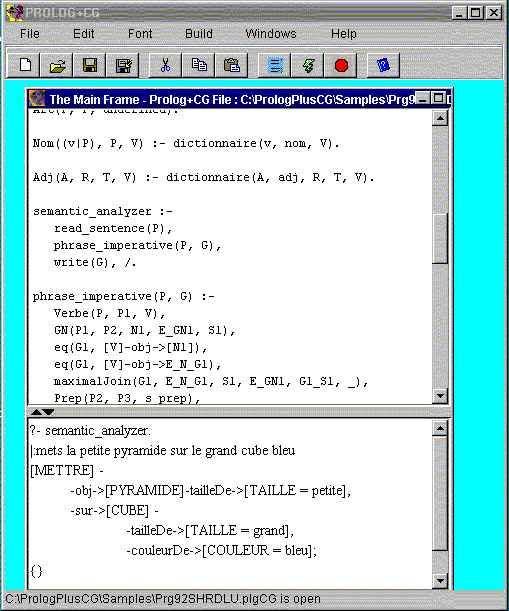
\includegraphics{snapshot1.png}
\end{center}
\caption{\label{PrologPlusCGEnvironment}PROLOG+CG Environment}
\end{figure}

\end{htmlonly}




Some of the commands/buttons of the environment are the following (the
others are the standards buttons for file and edition processing):


\includegraphics{compile.png} Compile a Prolog+CG File to produce an
object file (if it doesn't exist already)


\includegraphics{shortcut.png} Execute the interpreter to answer a
question


\includegraphics{help.png} Help

More information on the environment is provided in the next sections.

\subsection{Installation of PROLOG+CG}

Prolog+CG is implemented with JAVA 2. So the JRE of JAVA 2 should be
installed first. Then you have to download the PrologPlusCG ZIP file
and unzip it it somewhere on your harddrive (C for Windows for
instance). Inside the directory that this creates (e.g.,
``\texttt{PPCG}''), PrologPlusCG can be executed with the following
command (from the DOS Console):

\begin{center}
\texttt{java -classpath classes PrologPlusCG/PrologPlusCG}
\end{center}

\section{Elementary data types}\label{Sec:ElmentaryDataTypes}

Currently, the elementary data types are:

\begin{itemize}

  \item {\bf Number} (unsigned or negative integer or real : 23, -45,
    02.45, -564.675, etc.)

  \item {\bf Boolean} (true, false)

  \item A {\bf {\it string}} is any
sequence of characters surrounded by double-quotes.

Example: \texttt{"this is a string"}.

  \item A {\bf {\it constant identifier}} is any sequence of letters,
digits or underscore (\_) that begins with two letters.  

Examples of good identifiers: \texttt{pr32}, \texttt{papa},
\texttt{is\_good}, \texttt{pp34\_65}

Examples of illegal identifiers: \texttt{p45}, \texttt{\_rt},
\texttt{p\_rt}, \texttt{\_rrt}

\end{itemize}


\subsection{Variables}

The {\it identifier of a variable} can be either:

\begin{itemize}
  \item An underscore followed optionally by a
sequence of letters, digits or underscores.
  \item A letter.
  \item A letter followed by a digit or an
underscore, and followed optionally by a sequence of letters,
digits or underscores.
\end{itemize}

Examples of good variable identifiers:

\texttt{\_var1}, \texttt{\_}, \texttt{\_324}, \texttt{\_ce\_ci},
\texttt{x}, \texttt{x3}, \texttt{x\_var}

Note: The grammar of PROLOG+CG is given in Appendix
\ref{AppendixGrammar}.

\section{Composed data types overview}\label{Sec:ComposedDataTypes}

The composed data types of PROLOG+CG are: 

\begin{itemize}

  \item term, 

  \item list, 

  \item set, 

  \item concept and

  \item CG.

\end{itemize}

They are introduced in the next sections (sets and concepts are
considered in CG section, Section \ref{Sec:CG}).

\subsection{Example}

Figure \ref{HyperTextEditor} shows a simple Prolog+CG program that
introduces the basic data types of Prolog+CG: the program contains the
fact ``\texttt{prologCGData}'' that has one argument: a list of
different elements: an integer, a constant identifier, a string, a
boolean, a image file name (see the remark below), a list, a predicate
or term and a conceptual graph (CG). The program contains also a rule
that defines the goal ``\texttt{dataExple/1}'': it search the fact
``\texttt{prologCGData}'' and call the primitive goal
``\texttt{member}'' to access (with backtracking) all the elements
contained in the list.

The editor of Prolog+CG allows for some hypertext actions. For
instance, when the data is a file name of a multi-media data, like
``\texttt{ImgPrlg.png}'', the user can see the content of this file in
a separate window simply by selecting the whole name and by doing a
click on the left-button of the mouse. Figure \ref{HyperTextEditor}
shows the result of theses actions in the case
``\texttt{ImgPrlg.png}''.


\begin{latexonly}

\begin{figure}
\begin{center}
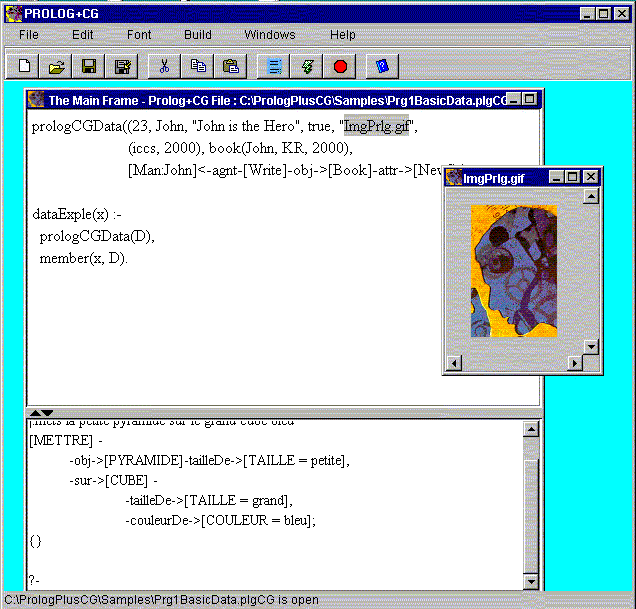
\includegraphics[scale=0.4]{MMDataEnv.png}
\end{center}
\caption{\label{HyperTextEditor}The ``hyper-text editor'' and basic data in PROLOG+CG}
\end{figure}

\end{latexonly}

\begin{htmlonly}

\begin{figure}
\begin{center}
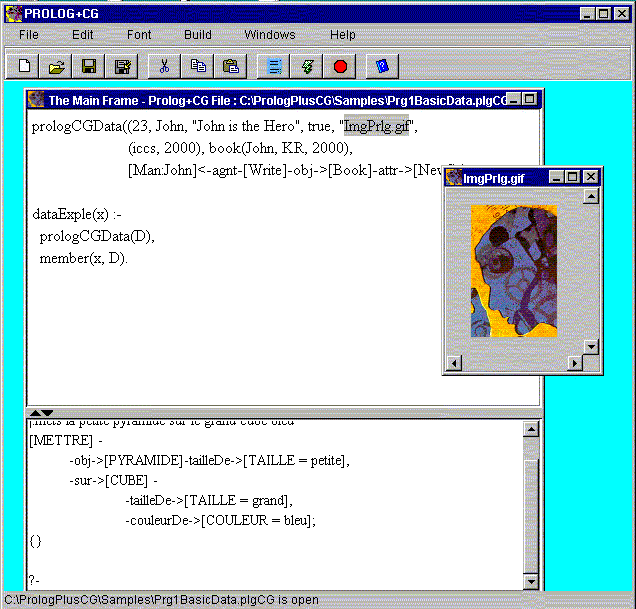
\includegraphics{MMDataEnv.png}
\end{center}
\caption{\label{HyperTextEditor}The ``hyper-text editor'' and basic data in PROLOG+CG}
\end{figure}

\end{htmlonly}


Now, to ask some questions about the above program, you first have to
compile it: choose ``\texttt{Build/Compile}'' from the menu or just
press on the corresponding button 
\includegraphics{compile.png}. Then
click in the bottom panel to switch to Console panel and write your
request just after the last prompt "\texttt{?-~}". To activate the
interpreter for responding to your request, press on the key
``\texttt{return/enter}'', or choose ``\texttt{Build/Answer
Question}'' or just press on the corresponding button

\includegraphics{shortcut.png}.

Here is the result of one question about the above program:


\begin{verbatim}
?- prologCGData(L).
{L = (23, John, "John is the Hero", false, "ImgPrlg.png", 
  (iccs,2000), book(John, KR, 2000),
      [Write]-
         -obj->[Book]-attr->[New],
         -agnt->[Man : John])}
?-
\end{verbatim}


\section{Term}\label{Sec:Term}

A term is an a
constant identifier followed optionally by a list of arguments.
An argument is either an elementary data
type, a variable or a composed data type.

\subsection{Examples of correct terms}


\begin{verbatim}
Prop4, 
Papa(Abdou), 
Publisher(Addison, "Conceptual Structure", 1984),
like(Kim, (banana, tomato, juice), 
     [Man: Kim]<-agnt-[Work]-manr->[Hard]),
phrase("kha eats banana", 
       st(np("kha"), vp(vb("eats"), np("banana"))),
       [Man:kha]<-agnt-[Eat]-obj->[Banana])
\end{verbatim}



\section{List}\label{Sec:List}

A list can be composed of zero, one or several elements separated
by comma. An element of a list is like an argument of a term; it is
either an elementary data type, a variable or a composed
data type.

{\bf Note:} Prolog+CG uses (parentheses) around lists rather than
[square brackets].  This is different from standard Prolog.

\subsection{Examples of correct lists}

\begin{verbatim}
(),
(tati),
(titi, 34, (356, ps(note(67), (2, 4)), "ha ha")),
(exp32, [Dat = (23, 12, 84)]<-birthOf-[Boy:Cham], 54)
\end{verbatim}


\section{Primitive operations}\label{Sec:PrimitiveOps}

Figure \ref{EnvPrimHier2} shows the window that is given to the user
when he asks for the primitives of the language, either by choosing
the menu action Help/Primitives or Windows/Primitives.  Each primitive
operation is given with its signature (number and types of the
arguments). In this section, we consider only the arithmetic,
relational, logical, list, stringIdent and multi-media primitive
operations. The other types of primitives are introduced later.


\begin{latexonly}

\begin{figure}
\begin{center}
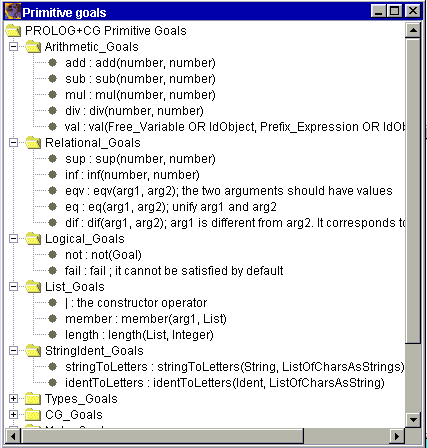
\includegraphics[scale=0.6]{EnvPrimHier2.png}
\end{center}
\caption{\label{EnvPrimHier2}Primitive operations}
\end{figure}

\end{latexonly}

\begin{htmlonly}

\begin{figure}
\begin{center}
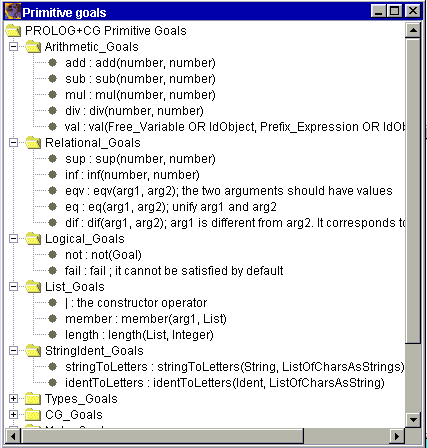
\includegraphics{EnvPrimHier2.png}
\end{center}
\caption{\label{EnvPrimHier2}Primitive operations}
\end{figure}

\end{htmlonly}


PROLOG+CG adopts a prefix notation to formulate an expression. Thus,
the infix expression: \texttt{3 + (4 - 5)} should be formulated in
PROLOG+CG as: \texttt{add(3, sub(4, 5))}. As shown below, the
primitive goal ``\texttt{val(Var, Expr)}'' evaluates the expression
Expr and associates its value to the variable Var. This is how
arithmetic computation is done in PROLOG+CG.

\begin{verbatim}
?- val(x, add(4, mul(5,3))).
{x = 19}
\end{verbatim}

{\bf Recall :} the request must terminates with a point (.) . To
activate the interpreter and get an answer, the user can either choose
the menu action ``\texttt{Build/Answer Question}'', or press the
button 
\includegraphics{shortcut.png}, or just press the
``\texttt{return}'' key on the keyboard. The interpreter returns

\begin{verbatim}
{x = 19}

?-val(x, mul(-4, add(6, 4.68))).

{x = -42.72}

?-eq(x, 34), val(y, div(765, x)).

{x = 34, y = 22.5}

?-eqv(x, 54).

Error: any variable in an expression should have a value.

\end{verbatim}

Note the difference between the two primitives ``\texttt{eq}'' and
``\texttt{eqv}'': {\bf eq} corresponds to the unification operation
while {\bf eqv} corresponds to the identity test; the two arguments of
{\bf eqv} should have a value.


\begin{verbatim}
?-eq(x, 54), eqv(x, 54).

{x = 54}

?-sup(43, -54).

{}

?-inf(-54, -34).

{}

?- eq(x, 34), eq(y, 54), dif(x, y).

{x = 34, y = 54}

?- eq(54, x), val(y, sub(56, 2)), not(eq(x, y)).

no.

?- eq(54, x), val(y, sub(56, 2)), not(dif(x, y)).

{x = 54, y = 54}

?- eq(papa(Hicham, x), papa(y,Nour)).

{x = Nour, y = Hicham}

?- eq((1, 2, 3, 4, 5),(x,y|z)).

{x = 1, y = 2, z = (3, 4, 5)}

?- dif(papa(Hicham, x), papa(y, Nour)).

no.

?- dif(papa(Hicham, x), papa(Wasouf, Nour)).

{}

\end{verbatim}



{\bf Note} the primitive goal {\bf dif(x,y)} is equivalent to :
{\bf not(eq(x,y))}.



\begin{verbatim}
?-fail.

no.

?-concat("xx", "yy", "xxyy").
  
{}

?-concat(X, "yy", "xxyy").
  
{X = "yy"}

?-concat("xx", Y, "xxyy").
  
{Y = "yy"}

?- concat("xx", "yy", Z).
  
{Z = "xxyy"}

?-stringToLetters("papa", L).

{L = ("p", "a", "p", "a")}

?-stringToLetters(x, ("m", "a", "i")).

{x = "mai"}

?-identToLetters(papa, L).

{L = ("p", "a", "p", "a")}

?-identToLetters(c, ("p", "a", "p", "i")).

{c = papi}

\end{verbatim}


\subsection{Examples of List operations}


\begin{verbatim}
?- member(3, (2, 3, 4, 5)).

{}

?- member(6, (2, 3, 4, 5)).

no.

?-member(x, (2, 3, 4)).

{x = 2}
{x = 3}
{x = 4}

?- length((4, 5, 6, 7), x).

{x = 4}

\end{verbatim}



\subsection{Multi-media primitives: show/2 and close/1}

Note: This is just a preliminary work on the integration of
multi-media in PROLOG+CG.

The following program illustrates this interesting aspect of the
language (sound and video will be integrated in the next version).
Again, please note that the text editor enables the user to see, in
auxiliary windows, the content of the media files: just select the
file name (without the double quotes) and do a click on a let-button
of the mouse. As shown in Figure \ref{MMPrg}, the program contains a
fact represented by a conceptual graph (CG) which states that
PrologPlusCG is a CGTool with an icon (represented by
``\texttt{ImgPrlg.png}''), a manual and a Java Code.

The rule that defines the goal ``\texttt{MMCGExample}'', searches for
the above fact, shows the image ``\texttt{ImgPrlg.png}'' in the window
``\texttt{wnd1}'' and shows the text file ``\texttt{DocTest.txt}'' in
the window ``\texttt{wnd2}''. It then waits for an input from the user
and then closes the two windows and writes a message. What is relevant
here is the use of the two primitive goals: ``\texttt{show/2}'' and
``\texttt{close/1}''.

\begin{itemize}

   \item {\bf show:} \texttt{show(Window\_Identifier, MMFileId\_String)}.

   \item {\bf close:} \texttt{close(Window\_Identifier)}

\end{itemize}


\begin{latexonly}

\begin{figure}
\begin{center}
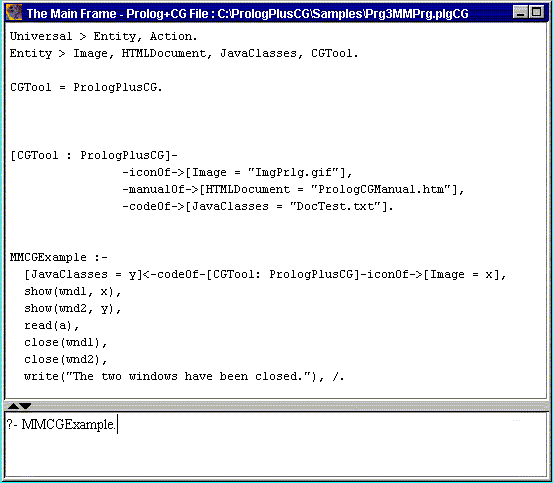
\includegraphics[scale=0.6]{MMPrg.png}
\end{center}
\caption{\label{MMPrg}A multi-media program}
\end{figure}

\end{latexonly}

\begin{htmlonly}

\begin{figure}
\begin{center}
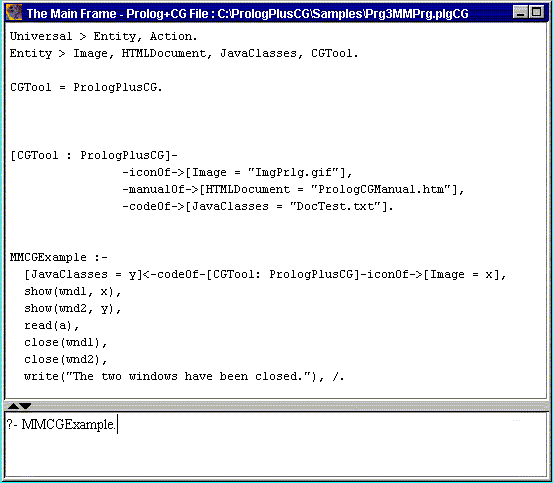
\includegraphics{MMPrg.png}
\end{center}
\caption{\label{MMPrg}A multi-media program}
\end{figure}

\end{htmlonly}


The interpretation of the request ``\texttt{MMCGExample.}'' by
PROLOG+CG gives the following result:

\begin{latexonly}

\begin{figure}
\begin{center}
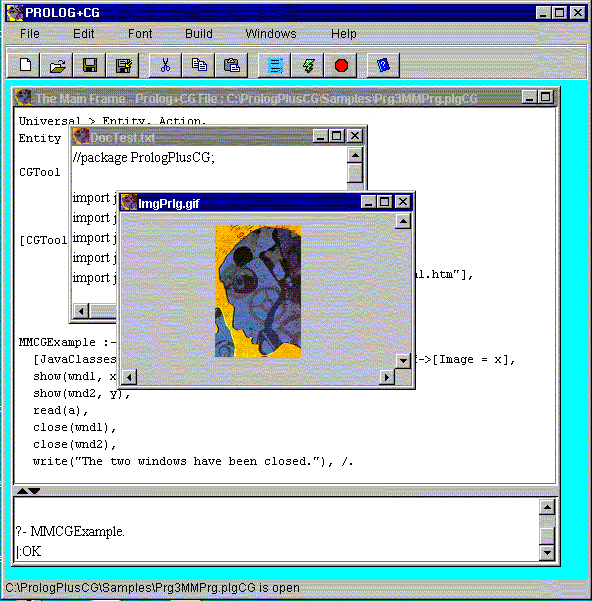
\includegraphics[scale=0.5]{MMPrgExec.png}
\end{center}
\caption{\label{MMPrgExec}Execution of the multi-media program}
\end{figure}

\end{latexonly}

\begin{htmlonly}

\begin{figure}
\begin{center}
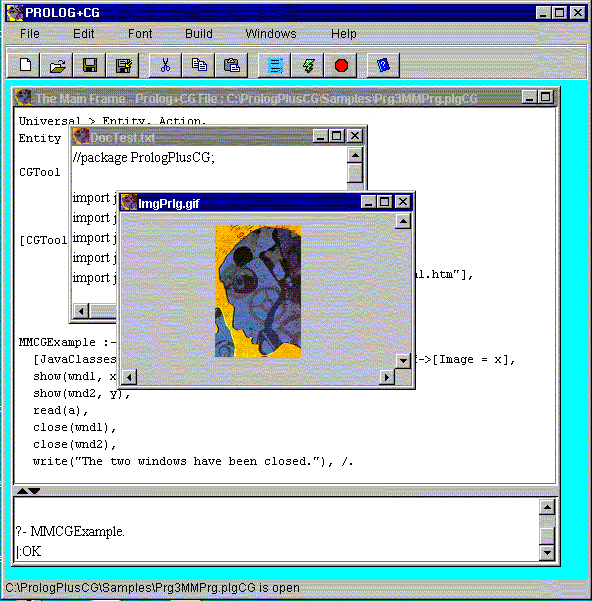
\includegraphics{MMPrgExec.png}
\end{center}
\caption{\label{MMPrgExec}Execution of the multi-media program}
\end{figure}

\end{htmlonly}



\section{Facts and inference Rules}\label{Sec:FactsAndRules}

As in PROLOG, a PROLOG+CG program is composed mainly of
{\it facts} and {\it inference rules}.

{\it {\bf A fact}} is a term or a CG followed by a
point. {\bf {\it An inference rule}} is composed of a
head and a tail, separated by the if symbol ``\texttt{:-}'' and it terminates
with a point. The {\it head} of a rule is a term or a CG and the
{\it tail} is a conjunction of elements, an element can be a term,
a CG or a variable. The next section gives a classic example of a
Prolog program, formulated in Prolog+CG without the use of CGs. In
later sections, we define CG and we present their use in Prolog+CG
programs.


\section{Samples I}\label{Sec:SamplesI}

The following program can be found in Samples/Others/Meal.prlg. It is
a classic example, proposed first by Colmerauer [Colmerauer, 85]. The
user can load the example (by opening the file Meal.prlg) and compile
it, or he can write and edit the program in the `Program pane'.



\begin{verbatim}
meal(a, r, m, d) :- 
        appetizer(a), 
        main(r, m), 
        val(x, add(3,4)), 
        dessert(d).

main(r, m) :- drink(r), principal(m).
main(r, m) :- drink(r), meat(m).

principal((m, m2)) :- fish(m), fish2(m2).

drink(Coke).
drink(Beer).

appetizer(radishes).
appetizer(pate).

fish(sole).
fish(tuna).

fish2(titi).
fish2(tata).

meat(pork).
meat(beef).

dessert(cake).
dessert(fruit).

little_sum(1, _x, _y) :- little_successor(_x, _y).
little_sum(_x1, _y, _z1) :- 
   little_successor(_x, _x1),
   little_sum(_x, _y, _z),
   little_successor(_z, _z1).

little_successor(1,2).
little_successor(2,3).
little_successor(3,4).
little_successor(4,5).
little_successor(5,6).
little_successor(6,7).
little_successor(7,8).
little_successor(8,9).

light_meal(a, m, d) :-
   meal(a, m, d),
   units(a, x),
   units(m, y),
   little_sum(x, y, u),
   units(d, z),
   little_sum(z, u, v).

// units with two arguments
units(beef, 3).
units(fruit, 1).
units(cake, 5).
units(pate, 6).
units(pork, 7).
units(radishes, 1).
units(sole, 2).
units(tuna, 4).



meal(a, m, d) :-
         appetizer(a),
\end{verbatim}


Once the editing task has been done, the user should compile the
program by pressing the button 
(or activating the menu action ``\texttt{Build/Compile}''). At this time, the
user can save the program (both the text format with the extension
.prlg and the object format with the extension .obj) and/or activates
the Console pane to ask questions.

Let us ask one question:

\begin{verbatim}
?- light_meal(a, m,d).

{a = radishes, m = sole, d = cake}
{a = radishes, m = sole, d = fruit}
{a = radishes, m = tuna, d = fruit}
{a = radishes, m = pork, d = fruit}
{a = radishes, m = beef, d = cake}
{a = radishes, m = beef, d = fruit}
{a = pate, m = sole, d = fruit}
\end{verbatim}


Next time, when the file is opened and
compiled directly; without any modification, the system will not
recompile it again, it will rather load the object file. But if the
text file is modified, the user should recompile and save
it.

\chapter{Ontologies and Conceptual Graphs}

\section{Specialization (Generalization)\label{Sec:SpecializationGeneralization}
rules}

Before considering {\it conceptual graphs} (CGs) in detail, we will
introduce two related notions: {\bf {\it concept types hierarchy}}
and{\bf {\it instantiation}}. The two constitute the {\it {\bf
support}} for the manipulation of CGs.  Indeed, as introduced later,
CG unification and the other CG operations make use of these
notions. Figure \ref{EnvPrimHierCG} gives the Prolog+CG primitives for
support and CGs manipulation.

\begin{latexonly}

\begin{figure}
\begin{center}
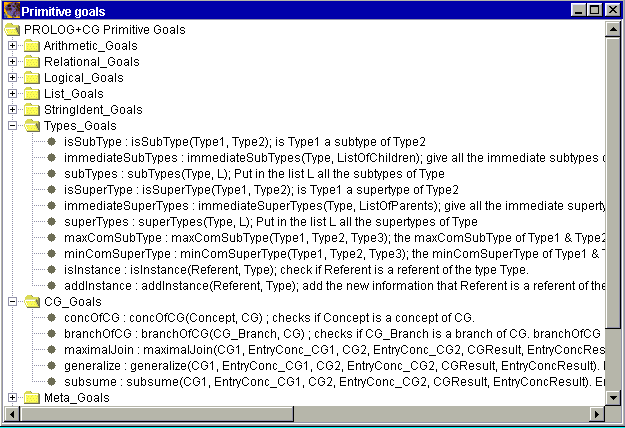
\includegraphics[scale=0.4]{EnvPrimHierCG.png}
\end{center}
\caption{\label{EnvPrimHierCG}Prolog+CG primitives for support and CG
manipulation}
\end{figure}

\end{latexonly}

\begin{htmlonly}

\begin{figure}
\begin{center}
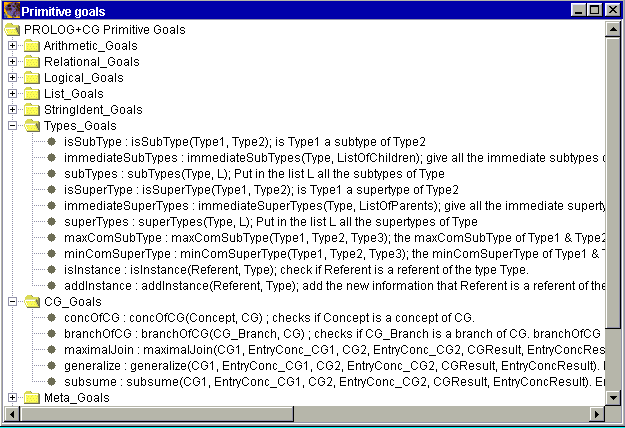
\includegraphics{EnvPrimHierCG.png}
\end{center}
\caption{\label{EnvPrimHierCG}Prolog+CG primitives for support and CG
manipulation}
\end{figure}

\end{htmlonly}


\subsection{Concept types hierarchy}

This describes the generalization/specialization relation between the
concept types used in the CGs. It encodes the famous ``\texttt{IsA}''
relation, used in many semantic network formalisms. In PROLOG+CG, a
concept type hierarchy is defined as a set of
{\bf {\it specialization rules}}. A specialization rule
describes the immediate subtypes Type1, Type2, \ldots{}, TypeN of a
type Type. It has the following form :

\begin{verbatim}
Type > Type1, Type2, ..., TypeN.
\end{verbatim}

\subsection{Example}


\begin{verbatim}
Universal > Person, Animal,
Action, Situation, Object, AbstractEntity, Attribute.
Person > Man, Woman.
Man > Boy, Employee.
Woman > Girl, Employee.
Employee > Supervisor.
Action > Drive, Love, Break, Rent, Begin, Press, Look.
Object > Vehicle, Machine, Key, Keyboard, Finger.
AbstractEntity > Society, Session, Years, Proposition.
Vehicle > Car, Truck.
Attribute > Fast, Color, Expensive, Big.
\end{verbatim}


\subsection{Operations on the concept types hierarchy} 

Currently, PROLOG+CG provides the following primitive operations on
concept type hierarchies:

\begin{itemize}

  \item {\bf isSubType(Type1,Type2):} checks if a type Type1
  is a subtype of a type Type2.

  \item {\bf immediateSubTypes(Type, L):} returns in the list L all
the immediate subtypes of a type Type.

  \item {\bf subTypes(Type, L):} returns in the list L all
  the subtypes of a type Type. The types are given in the
  breadth-first order.


  \item {\bf isSuperType(Type1, Type2):} checks if a type
  Type1 is a super-type of a type Type2.

  \item {\bf immediateSuperTypes(Type, L):} returns in the
  list L all the immediate super-types of a type Type.

  \item {\bf superTypes(Type, L):} returns in the list L all
  the super-types of a type Type. The types are given in the
  breadth-first order.

  \item {\bf maxComSubType(Type1, Type2, T):} gives in T the
  maximum common subtype of the types Type1 and Type2.

  \item {\bf maxComSubTypes(Type1, Type2, L):} gives in L the
  list of ``maximal common subtypes''.  If the type hierarchy is not a
  strict lattice, this can be useful.  If it is a strict lattice, then
  this is the same as maxComSubType, except that a list is returned
  (with only one element).  The ``maximum common subtypes'' is defined
  as follows: If Type1 is a subtype of Type2, or vice versa, then the
  one that is the subtype is returned as the single element of the
  list.  Otherwise, what is returned is the list of those common
  subtypes that do not have any supertypes in the list of all common
  subtypes of types Type1 and Type2.

  \item {\bf minComSuperType(Type1, Type2, T):} gives in T
  the minimum common super-type of the types Type1 and Type2.

  \item {\bf maxComSubTypes(Type1, Type2, L):} gives in L the
  list of ``minimal common supertypes''.  If the type hierarchy is not a
  strict lattice, this can be useful.  If it is a strict lattice, then
  this is the same as minComSuperType, except that a list is returned
  (with only one element).  The ``minimum common supertypes'' is defined
  as follows: If Type1 is a supertype of Type2, or vice versa, then
  the one that is the supertype is returned as the single element of
  the list.  Otherwise, what is returned is the list of those common
  supertypes that do not have any subtypes in the list of all common
  supertypes of types Type1 and Type2.

\end{itemize}

\subsection{Examples}


\begin{verbatim}
?- isSubType(Supervisor, Person).

{}

?-isSubtype(Supervisor, Girl).

no.

?-immediateSubTypes(Action, L).

{L = (Drive, Love, Break, Rent, Begin, Press, Look)}

?-subTypes(Person, L).

{L = (Man, Woman, Boy, Employee, Girl, Supervisor)}

?-isSuperType(Person, Supervisor).

{}

?-immediateSuperTypes(Employee, L).

{L = (Man, Woman)}

?-superTypes(Employee, L).

{L = (Man, Woman, Person, Universal)}

?- maxComSubType(Man, Woman, x).

{x = Employee}

?-maxComSubType(Person, Employee, x).

{x = Employee}

?-minComSuperType(Supervisor, Boy, x).

{x = Man}
\end{verbatim}



\section{Instantiation rules}\label{Sec:Instantiation}

The instantiation relation relates an instance to its type. In
PROLOG+CG, {\bf instances of a type} are described with an
{\bf {\it instantiation rule}}:

\begin{verbatim}
Type = Inst1, Inst2, ..., InstN.
\end{verbatim}

Instantiation rules are specified as a complement to the
specialization rules which describe the concept type hierarchy.

\subsection{Examples}

(we assume the concept type hierarchy introduced in Section
\ref{Sec:SpecializationGeneralization}):


\begin{verbatim}
Boy = John, Bob, Sam, Andre.
Girl = Sue, Mary.
Color = red.
Machine = res23.
Years = four.
Key = enter.
\end{verbatim}


\subsection{Operations on instances} 

PROLOG+CG provides two operations on type instances (figure
\ref{EnvPrimHierCG}):

\begin{itemize}
  \item {\bf isInstanceOf(Referent, Type):} checks if the
  referent Referent is an instance of a type Type.

  \item {\bf addInstance(Referent, Type):} adds Referent as a
  new instance in the instances declaration of the type Type.

\end{itemize}

\subsection{Examples}


\begin{verbatim}
?- isInstance(Sue, Girl).

{}

?-isInstance(Sue, Person).

{}

?-isInstance(Sue, Boy).

no.

?-isInstance(Karl, Boy).

no.

?-addInstance(Karl, Boy).

{}

?- addInstance(Emp01, Employee).

{}
\end{verbatim}



Note that following the two above operations, the instantiation rule
for the type ``\texttt{Boy}'' is modified and a new instantiation rule
is added for the type ``\texttt{Employee}'':

\begin{verbatim}
Boy = John, Bob, Sam, Andre, Karl.
Girl = Sue, Mary.
Color = red.
Machine = res23.
Years = four.
Key = enter.
Employee = Emp01.


(continue ...)


?-isInstance(Karl, Boy).

{}

?- isInstance(Karl, Person).

{}

?-
\end{verbatim}



\section{Conceptual Graphs (CG)}\label{Sec:CG}

As noted earlier, a composed data item in PROLOG+CG can be a term,
a list, a {\bf {\it concept}} or a
{\it {\bf conceptual graph (CG)}.}

\begin{itemize}

  \item {\bf CG.} A conceptual graph (CG), in Prolog+CG, is a graph of
nodes that represent {\it concepts} and that are related by {\it
conceptual relations}.

  Only binary relations are possible (this constraint is for
simplicity and practical purpose only).

{\it {\bf Remark:}} Prolog+CG provides a large
flexibility in the use of variables inside CG: a variable can stand
for:

 \begin{itemize}

  \item  a whole CG,

  \item a whole concept (like: {\tt [Man]-agnt->X} ; X is
a variable),

  \item a relation (like: {\tt [Man]-R->[Eat]} ; R is a
variable),

  \item a concept type or a concept referent (like: {\tt [A :
B]-agnt->[Eat]} ; A and B are variables).

\end{itemize}

Such a flexible use of variables enhances the expressive power of
the language, according to CG manipulation.



\item {\bf Concept.} A concept is composed of a type, an
optional referent and an optional description.

  \begin{itemize}

  \item A concept type can be a variable or an identifier that refers to
a type defined in the concept type hierarchy.

  \item A concept referent can be a variable, an instance (an identifier
or a string) declared in instances declaration rules, a set of
instances, a co-referent (represented by a variable) or a
multi-referent. 

  \item A concept description is any Prolog+CG data: an elementary data
like an integer, a real, a boolean, an identifier, a string or a
composed data like a list, a term, a concept or a CG.

\end{itemize}



\end{itemize}

A multi-referent has the form {\bf ``\texttt{*Number}''} and it is
only used in the linear notation to identify all occurrences of a
concept. A multi-referent is not represented in the internal
representation of the concept. Examples are given below.

\subsection{Concept and CG Linear Notation}

The linear notation used in PROLOG+CG to express CG is similar to
the notation introduced first by Sowa. As introduced above, a concept
has tree fields surrounded by brackets.

\subsubsection{Examples of concepts}

\begin{verbatim}
[Man], 
[Man : John],
[Man : {John, Carl, Henry}], 
[Cat : x], 
[Human : *1], 
[Integer = 25], 
[List = (1, 2, 3)],
[Date : CurrentDate = (04,01,2000)],
[Term = papa(x, Hicham)],
[Proposition :propHenry = [Man : Carl]<-agnt-
            <-[Think]-obj->[Proposition =
                           [Man: Carl]-attr->[Crazy] ] ]
\end{verbatim}


A relation R between two concepts C1 and C2 can be expressed as
follows:

\begin{verbatim}
[C1]-R->[C2]
\end{verbatim}

R of C1 is C2, or \texttt{[C2]<-R-[C1]} which is the same.

\subsubsection{Example of a simple CG:}


\begin{verbatim}
[Girl : Fouzia]<-agent-[Walk]

agent of Walk is Girl Fouzia.
\end{verbatim}

If a concept is connected to several relations, writes the concept,
then a dash followed by a sequence of relations description separated
by comma (see the Appendix for the detailed
definition of CG grammar). Also, the CGs given in this manual
illustrates several cases of writing CG.

\subsubsection{Example of CG --- continued}

\begin{verbatim}
[Extract]-
    -agnt->[Person],
    -obj->[Text],
    -target->[Book].
\end{verbatim}

{\it {\bf The role of the hyphen ``\texttt{-}'', the comma
``\texttt{,}'' and the semi-colon ``\texttt{;}'':}} if a concept (like
{\bf [Extract]}) has several branches connected to it, then write the
``\texttt{-}'' after the concept, write the branches using
``\texttt{,}'' to seperate between them, and use the ``\texttt{;}'' at
the end to indicate the end of the specification of the branches. In
this sense, the branches of a concept are enclosed by two delimiters:
``\texttt{-}'' and ``\texttt{;}'' and they are separated by the
delimiter ``\texttt{,}''. Note that the delimiter ``\texttt{;}'' is
optional if we are at the end of the CG, like the example above.Of
course, a concept at the end of a relation can be connected itself to
other relations and so on, forming a tree (and a graph as described
below). This case is illustrated by the following example :

\subsubsection{Example}


\begin{verbatim}
[Work]-
      -agnt->[Person: Jane]-
                              -ageOf->[Age = 30],
                              <-poss-[House : *1];,
      -near->[House : *1].
\end{verbatim}


In the example above, the delimiter ``\texttt{;}'' is used to specify
the end of the specification of the branches of {\bf [Person : Jane]}
and the delimiter ``\texttt{,}'' that follows ``\texttt{;}'' is used
to separate between the two branches of {\bf [Work]}.

Finally, note that the indentation and carriage-return are used only
for ``pretty-print''; they are not significant in the analysis of the
notation.

A linear formulation of any graph (and hence, of a CG) provides in
general a way to specify several occurrences of the same node (the
same concept for CG). In PROLOG+CG, a referent and/or a multi-referent
is used for this end. In the above example, the multi-referent
``\texttt{*1}'' is used to specify that the two concepts {\bf [House :
*1]} and {\bf [House : *1]} are in fact two occurrences of the same
concept.

Relations that are connected to a concept
can be specified as relations connected to the occurrences of the
same concept.

\subsubsection{Example}

\begin{verbatim}
[Extract]-
    -agnt->[Person],
    -obj->[Inanimate : *1]-matr->[Wood],
    -manr->[Strong],
    -target->[Inanimate]-on->[Inanimate :
*1]-priceOf->[Expensive].
\end{verbatim}

\subsubsection{Example of compound CG}

\begin{verbatim}
[Person]<-agnt-[Perform]-obj->[Action = [Eat]-
           -obj->[Walnut = wal2]-part->[Shell:myShell = toto],
           -instr->[Spoon]-matr->[Shell : myShell]
]-instr->[Roulette].
\end{verbatim}

Maybe a better formulation is as follows:

\begin{verbatim}
[Action = [Eat]-
           -obj->[Walnut = wal2]-part->[Shell : myShell = toto],
           -instr->[Spoon]-matr->[Shell : myShell]
]<-obj-[Perform]-
           -agnt->[Person],
           -instr->[Roulette].
\end{verbatim}

Note that the two concepts ``{\bf [Shell : myShell = toto]}'' and
``{\bf [Shell : myShell]}'' are the same. They are identified by the
referent ({\bf myShell}). Thus, when the concept has a specific
referent, this can be used (instead of a multi-referent) to specify
the identity of several occurrences of the same concept.

\subsection{Co-references}

A {\it {\bf Co-reference}} is represented with a
variable. An example will illustrate this important notion:


\begin{verbatim}
[Man : x]<-agnt-[Begin]-srce->[Proposition = 
                  [Person]<-pat-[Look]-dest->[Person : x] ]
\end{verbatim}

The variable x plays a role of a co-reference between the two
concepts {\bf [Man : x]} and {\bf [Person : x]}.
Thus, the two concepts refere to the same entity.

With the above illustrations concerning CG notation, the user can
combine them in order to formulate any CG.

\subsection{The use of CG in PROLOG+CG}

In PROLOG+CG, CG is a basic data structure, like a term or a
list. CG can be an argument of a term, an element in a list, a value
of a concept, the head of a rule (or a fact) or a goal in the tail of
a rule.

\section{Samples II}\label{Sec:SamplesII}

To illustrate the use of CG in PROLOG+CG, we give two programs in this
section. The first has been proposed first by Fargues et al. [6]
(which is a Prolog-based formulation of an example presented by Sowa,
using Peirce Logic). In the first program, all the goals are
formulated as CGs. In general however, we can have in one rule some
goals that are represented by CGs and others that are represented by
terms. The second program illustrates this point.

\subsection{Program 1}

(it can be found in Samples/Others/Citizen.prlg)


\begin{verbatim}
Universal > PERSON, BORN, NATURALIZE, COUNTRY.
PERSON > CITIZEN, GIRL.

GIRL = "Dorothy".
PERSON = "Tinman".
COUNTRY = "Oz".

[CITIZEN : x]<-MEMB-[COUNTRY : "Oz"] :-
   [PERSON: x]<-AGNT-[BORN]-LOC->[COUNTRY : "Oz"].

[CITIZEN : x]<-MEMB-[COUNTRY : "Oz"] :-
   [PERSON: x]<-CHLD-[PERSON: y], 
   [CITIZEN : y]<-MEMB-[COUNTRY : "Oz"].

[CITIZEN : x]<-MEMB-[COUNTRY : "Oz"] :-
   [PERSON : x]<-RCPT-[NATURALIZE]-LOC->[COUNTRY : "Oz"].

[PERSON : "Tinman"]-
    -CHLD->[GIRL : "Dorothy"], 
    <-AGNT-[BORN]-LOC->[COUNTRY : "Oz"].
\end{verbatim}


Let us ask some queries:


\begin{verbatim}
?- [CITIZEN : x]<-MEMB-[COUNTRY : y].

{x = "Tinman", y = "Oz"}.

?- [CITIZEN : "Dorothy"]<-MEMB-[COUNTRY : "Oz"].

no.
\end{verbatim}


\subsection{Program 2}

(it can be found in Samples/Others/GoodSister.prlg):


\begin{verbatim}
Universal > Person, Action, Object, Attribute. 
Object > House, Restaurant, Walnut, Shell, Spoon. 
Attribute > Classical, Age, Easily. 
Person > Man, Woman. 
Action > Perform, Go, Work, Buy, Eat, Search. 

Man = Jo, Mark. 
Woman = Mary, Jane. 

// Prolog+CG rules. Notes that a goal can be a term or a CG. 
// x, w and a are variables. 
goodSister(x) :- 
       employee(x), 
       [Woman : x]-attr->[Classical]. 

[Woman : w]-attr->[Classical] :- 
       [Work]-
             -near->[House]-poss->[Woman : w]-ageOf->[Age = a], 
             -agnt->[Woman : w], 
       inf(a, 40).

// *1 is a multi-referent. 
[Work]- 
      -agnt->[Person : Jane]-
                 -ageOf->[Age = 30], 
                 <-poss-[House : *1]<-nearOf-[Restaurant];, 
      -near->[House : *1].


employee(Mary). 
employee(Jane). 


// An example of compound CG 
[Person]<-agnt-[Perform]-obj-> 
   [Action = [Eat]-
     -obj->[Walnut=wal2]-part->[Shell:myShell = toto], 
     -instr->[Spoon]-matr->[Shell : myShell] 
   ]-manr->[Easily].


sense("extract", [Search]- 
                         -agnt->[Person], 
                         -from->[Book], 
                         -obj->[Information]). 


sense("classical woman", [Woman]-attr->[Classical]). 
\end{verbatim}


Let us consider now some queries:


\begin{verbatim}
?- goodSister(x).
 
{x = Jane}

?-goodSister(Mary).
  
 no.

?- [Woman: x]-attr->[Classical].
 
{x = Jane}
\end{verbatim}

The next two queries illustrate how the compound CG are naturally
expressed and manipulated in PROLOG+CG (like simple CG). Note that an
embedded CG is considered in PROLOG+CG as a {\it value} of the
concept ({\it not as a referent}).


\begin{verbatim}
?- [Man]<-agnt-[Perform]-obj->[Action = 
        [Eat]-obj->[Walnut]-part->[Shell : x] ].

{x = myShell}

?- [Man]<-agnt-[Perform]-obj->[Action = x].
{x = [Eat]-
       -obj->[Walnut = wal2]-part->[Shell:myShell = toto]-
               <-matr-[Spoon : *1];,
       -instr->[Spoon : *1]}

?- sense("extract", g).

{g = [Search]-
          -agnt->[Person],
          -from->[Book],
          -obj->[Information]}
\end{verbatim}


In the next request, the variable x stand for the concept
type. Thus we can reason and manipulate all the fields of a concept
(the type, the referent and the value).


\begin{verbatim}
?- sense("extract", [x]<-obj-[Action]-agnt->[Person]).

{x = Information}

?- sense("extract", [x]<-obj-[Work]-agnt->[Person]).

no.
\end{verbatim}


The following query is interesting: the second goal is a variable that
will be unified, after the satisfaction of the first goal, to a CG. So
the request is to search the CG associated to ``classical woman'' and
then try to solve it (as the next goal of the request).


\begin{verbatim}
?- sense("classical woman", g), g.

{g = [Woman]-attr->[Classical]}
\end{verbatim}


\section{CG operations}\label{Sec:CGOps}

Actually, PROLOG+CG provides the following operations on CG, for both
simple and compound CG with sets and co-references (Figure
\ref{EnvPrimHierCG}):

\begin{itemize}

  \item {\bf concOfCG(c, g):} check if c is a concept of the CG
g. Concept unification is used to search for such a concept.  The
primitive ``\texttt{concOfCG/2}'' is non-deterministic: it searchs by
default for all the concepts in the CG g that could unify the concept
c which could be totally determined, partially specified (the concept
type or referent is a variable) or non-specified (a variable). If c is
a free variable then the primitive, with the backtrack, will return
all the concepts of the CG g.

  \item {\bf branchOfCG(b, g):} check if the branch b (a branch is two
concepts connected by a relation) is a branch of the CG g. The
primitive is non-deterministic: it searches by default for all the
branches in the CG g that could unify the branch b which could be
totally determined, partially specified or non-specified (a
variable). If b is a free variable then the primitive, with the
backtrack, will return all the branches of the CG g.

  \item {\bf maximalJoin(g1, g2, g3)}: returns in g3 the maximal join
of the two CG g1 and g2. maximalJoin joins in g3 any information
contained in g1 and g2. The join is guided of course by the matching
of the two graphs g1 and g2.

  \item {\bf generalize(g1, g2, g3)}: returns in g3 the generalization
of the two CG g1 and g2. generalize puts in g3 the common information
found in g1 and g2. Again, the generalize operation is guided by the
matching of the two CG.

  \item {\bf subsume(g1, g2)}: checks that g1 subsumes g2 ; checks
that g1 is more general than g2. subsume checks that the information
contained in g1 is more general than the information contained in g2.

  \item {\bf subsume(g1, g2, g3)}: checks that g1 subsumes g2
and return in g3 the image of g1 in g2 (the sub-graph of g2 that is
ismorph to g1).

\end{itemize}

These operations are provided also with entry points which are very
usefull in natural language processing, as illustrated in section
\ref{Sec:SampleIII} (sample III).

\subsection{Examples of calling CG operations}

(it can be found in Samples/ExpleCGs.prlg)

To facilitate the demo, the program contains already the specification
of some CGs.


\begin{verbatim}
Universal > Person, Animal, Action, Situation, Object, 
            AbstractEntity, Attribute.
Person > Man, Woman, Employee.
Man > Boy.
Woman > Girl.
Employee > Supervisor.
Action > Drive, Love, Break, Rent, Begin, Press, Look.
Object > Vehicle, Machine, Key, Keyboard, Finger.
AbstractEntity > Society, Session, Years, Proposition.
Vehicle > Car, Truck.
Attribute > Fast, Color, Expensive, Big.

Boy = John, Bob.
Girl = Sue, Mary.
Color = red.
Machine = res23.
Years = four.
Key = enter.

// cg(cg12, g1, g2) , maximalJoin(g1, g2, g3).
cg(cg12, [Person]<-agnt-[Drive]-obj->[Car],
         [Boy: John]<-agnt-[Drive]-manr->[Fast]).

// cg(cg34, g1, g2) , generalize(g1, g2, g3).
cg(cg34, [Boy: John]<-agnt-[Drive]-obj->[Car]-chrc->[Color: red],
         [Girl: Sue]<-agnt-[Drive]-
                              -obj->[Truck],
                              -manr->[Fast]).

// cg(cg56, g1, g2) , subsume(g2, g1).
// cg(cg56, g1, g2) , subsume(g2, g1, g3).
cg(cg56, [Man: John]-child->[Boy: Bob]<-agnt-[Love]-
                         ->obj->[Girl: Mary],
         [Person]-child->[Person]).
cg(cg70, [Break]-
             -agnt->[Employee],
             -obj->[Machine]-attr->[Expensive],
         [Situation]-mainActOf->[Break]-
                      -agnt->[Supervisor],
                      -obj->[Machine: res23]-qlte->[Big]).

// cg(cg910, g1, g2) , maximalJoin(g1, g2, g3).
cg(cg910,
       [Person: John]<-agnt-[Begin]-
                      -obj->[Session],
                      -srce->[Proposition = 
                   [Person: John]<-agnt-[Press]-
                      ->obj->[Key: enter]-part->[Keyboard] ];,
      [Man]<-agnt-[Begin]-srce->[Proposition = 
                   [Person]<-agnt-[Press]-
                           -obj->[Key],
                           -manr->[Fast] ]).

// cg(cg1011, g1, g2) , maximalJoin(g1, g2, g3).
cg(cg1011,
   [Person]<-agnt-[Begin]-
             -obj->[Session],
             -srce->[Proposition =
                 [Person]<-agnt-[Press]-obj->[Key: enter]-
                             ->part->[Keyboard] ],
       [Man]<-agnt-[Begin]-srce->[Proposition = 
             [Person]<-pat-[Look]-dest->[Person] ]).
\end{verbatim}




Let us asks some queries:

\subsubsection{Examples of calling the primitive concOfCG/2}

\begin{verbatim}
?- concOfCG([Drive], [Drive]-obj->[Car]).

{}

?- concOfCG(c, 
            [Man : John]-child->[Boy : Bob]-
                     <-agnt-[Love]-obj->[Girl : Mary]).
{c = [Man : John]}
{c = [Boy : Bob]}
{c = [Love]}
{c = [Girl : Mary]}

?- concOfCG([Person : x], 
            [Man : John]-child->[Boy : Bob]-
                  <-agnt-[Love]-obj->[Girl : Mary]).
{x = John}
{x = Bob}
{x = Mary}
\end{verbatim}


\subsubsection{Examples of calling the primitive branchOfCG/2}

{\it Gives the children of the person x}: note that the whole concept
(the target of the relation child) is represented by the variable C.


\begin{verbatim}
?- branchOfCG([Person : x]-child->C, 
              [Man : John]-
                          -child->[Boy : Bob],
                          -attr->[Color :black],
                          -child->[Girl : Mary],
                          <-agnt-[Eat] ).

{x = John, C = [Boy : Bob]}
{x = John, C = [Girl : Mary]}
\end{verbatim}


{\it Search the relations that relate two persons x and y}: note that
the relation is represented by a variable.


\begin{verbatim}
?- branchOfCG([Person : x]-R->[Person : y], 
            [Man : John]-
                        -child->[Boy : Bob],
                        -attr->[Color :black],
                        -child->[Girl : Mary],
                        <-agnt-[Eat]
                        ).

{x = John, R = child, y = Bob}
{x = John, R = child, y = Mary}
\end{verbatim}


{\it Gives all the branches of a CG:}

\begin{verbatim}
?- branchOfCG(b, [Man : John]-
                             -child->[Boy : Bob],
                             -attr->[Color :black],
                             -child->[Girl : Mary],
                             <-agnt-[Eat] ).

{b = [Man : John]-child->[Boy : Bob]}
{b = [Man : John]-attr->[Color : black]}
{b = [Man : John]-child->[Girl : Mary]}
{b = [Eat]-agnt->[Man : John]}
\end{verbatim}


\subsection{Unification}

{\bf eq/2} is the unification operator.

\begin{itemize}

  \item {\bf eq(Concept c1, Concept c2)}and
  {\bf eq(CG g1, CG g2):}

\end{itemize}


\subsubsection{Unification on concepts}

Concepts are considered to be Prolog+CG data structures on a par
with all other data structures.


\begin{verbatim}
?- eq([Person : John], [Man : x]).

{x = John}

?- eq([Person : John], [Woman : x]).

no.

? member([Person : x], 
         ([Man : John], [Color : red], [Woman : Mary])).

{x = John}
{x = Mary}
\end{verbatim}



\subsubsection{Unification on simple CGs with sets}

It fails since Andre is not specified in the set \{John, Bob, Sam\}.


\begin{verbatim}
?- eq([Person : Andre]<-agnt-[Drive]-obj->[Vehicle : myCar],
      [Boy : {John, Bob, Sam}]<-agnt-[Drive]-
                                               -obj->[Car :x],
                                               -manr->[Fast]).

no.

?- eq([Person : Bob]<-agnt-[Drive]-obj->[Vehicle : myCar],
      [Boy : {John, Bob, Sam}]<-agnt-[Drive]-
                                               -obj->[Car :x],
                                               -manr->[Fast]).
{x = myCar}
\end{verbatim}





\subsubsection{Unification on compound CGs with co-referents}

The unification succeeds since, apart from the unification of the
other components of the two CGs, the co-reference `x' between {\bf
[Person : x]} and {\bf [Man : x]} in the first CG can be unified with
the co-reference `Andre' between {\bf [Man : Andre]} and {\bf [Boy :
Andre]} in the second CG. Indeed, the concepts {\bf [Person : x]}/{\bf
[Man : x]} refer to the same entity and this is also the case for the
concepts {\bf [Man : Andre]}/{\bf [Boy : Andre]}.


\begin{verbatim}
?-eq([Person : x]<-agnt-[Begin]-srce->[Proposition = 
             [Man : x]<-agnt-[Action]-obj->[Object]],
     [Man : Andre]<-agnt-[Begin]-
             -obj->[Session],
             -srce->[Proposition = 
                  [Boy:Andre]<-agnt-[Press]-
                      ->obj-> [Key :enter]-part->[Keyboard]]).

{x = Andre}
\end{verbatim}





\subsubsection{Unification on compound CGs with co-referents}

here, the unification fails since the co-reference `x' in the first CG
can't be unified.


\begin{verbatim}
?- eq([Person : x]<-agnt-[Begin]-srce->[Proposition = 
            [Man : x]<-agnt-[Action]-obj->[Object]],
      [Man : Andre]<-agnt-[Begin]-
            -obj->[Session], 
            -srce->[Proposition = 
                [Boy : John]<-agnt-[Press]-
                     -> obj->[Key:enter]-part->[Keyboard]]).

no.
\end{verbatim}



\subsubsection{Unification on compound CGs with co-referents}

here, the unification fails too since the co-reference `x' in the
first CG has no corresponding co-reference in the second CG.



\begin{verbatim}
?- eq([Person : x]<-agnt-[Begin]-srce->[Proposition = 
          [Man : x]<-agnt-[Action]-obj->[Object]],
      [Man]<-agnt-[Begin]-
          -obj->[Session],
          -srce->[Proposition =
                [Boy]<-agnt-[Press]-
                      ->obj->[Key : enter]-part->[Keyboard]]).

no.
\end{verbatim}





\subsection{Subsume operation}


\begin{verbatim}
?- subsume(
      [Person]-child->[Person],
      [Man:John]-child->[Boy:Bob]<-agnt-[Love]-obj->[Girl:Mary]).

{}

?- subsume(
    [Person]-child->[Person],
    [Man:John]-child->[Boy:Bob]<-agnt-[Love]-obj->[Girl:Mary],
    g3).

{g3 = [Man :John]-child->[Boy : Bob]}
\end{verbatim}





\subsubsection{Subsume on simple CGs with sets}


\begin{verbatim}
?- subsume([Person]-child->[Person : {John, Sam}],
           [Man : John]-child->[Boy : {Bob, John, Andre, Sam}]-
                <-agnt-[Love]-obj->[Girl : Mary]).

{}
\end{verbatim}


\subsubsection{The same request but we specify the third argument to get the
image of the first argument}


\begin{verbatim}
?- subsume(
     [Person]-child->[Person : {John, Sam}],
     [Man : John]-child->[Boy : {Bob, John, Andre, Sam}]-
              <-agnt-[Love]-obj->[Girl : Mary];, 
     g).

{g = [Man : John]-child->[Boy : {Bob, John, Andre, Sam}]}
\end{verbatim}






\subsubsection{Subsume fails since the set {John, Sam} is not included in the set \{Bob, John, Andre\}}



\begin{verbatim}
?-subsume(
     [Person]-child->[Person : {John, Sam}],
     [Man : John]-child->[Boy : {Bob, John, Andre}]-
             <-agnt-[Love]-obj->[Girl : Mary]).

no.
\end{verbatim}





\subsubsection{Subsume on compound CGs without co-references}


\begin{verbatim}
?- subsume(
     [Person ]<-agnt-[Begin]-srce->[Proposition = 
              [Person]<-agnt-[Action]-obj->[Object]],
     [Man]<-agnt-[Begin]-
              -obj->[Session],
              -srce->[Proposition =
                 [Boy]<-agnt-[Press]-
                    ->obj->[Key:enter]-part->[Keyboard]];,
     g).

{g = [Begin]-
            -srce->[Proposition = [Press] -
                                             -obj->[Key : enter],
                                             -agnt->[Boy]],
            -agnt->[Man]}
\end{verbatim}





\subsubsection{Subsume on compound CGs with co-reference}

The same request as the precedent but a co-reference `x' is added
in the first argument. Subsume fails in this case since the
co-reference `x' is not mapped to a co-reference in the second CG :
the first CG doesn't totally subsume the second CG; the information
that the two concepts [Person : x] and [Person : x] refers to the same
entity is not found in the second CG since the corresponding concepts
in the second CG [Man] and [Boy] could refer to different
entities.


\begin{verbatim}
?- subsume(
    [Person :x]<-agnt-[Begin]-
          ->srce->[Proposition = 
                    [Person:x]<-agnt-[Action]-obj->[Object]];,
    [Man]<-agnt-[Begin]-
          -obj->[Session],
          -srce->[Proposition =
                    [Boy]<-agnt-[Press]-
                        ->obj->[Key:enter]-part->[Keyboard]];,
    g).

no.
\end{verbatim}






\subsubsection{Subsume on compound CGs with co-reference}

The same request as the precedent but a co-reference `y' is added
to the second CG. Subsume is possible in this case since the
constraint imposed by the co-reference in the first CG is verified by
a corresponding co-reference in the second CG.


\begin{verbatim}
?- subsume([Person :x]<-agnt-[Begin]-srce->[Proposition =
           [Person:x]<-agnt-[Action]-obj->[Object]],
           [Man : y]<-agnt-[Begin]-
                -obj->[Session],
                -srce->[Proposition =
                        [Boy: y]<-agnt-[Press]-
                          ->obj->[Key :enter]-part->[Keyboard]];, 
           g).

{x = FREE, 
 y = FREE, 
 g = [Begin] -
             -srce->[Proposition = [Press] -
                           -agnt->[Boy : y],
                           -obj->[Key : enter]],
                           -agnt->[Man : y]
\end{verbatim}






\subsection{maximalJoin operation}


\begin{verbatim}
?- cg(cg12, g1, g2), maximalJoin(g1, g2, g3).

{g1 = [Drive] -
              -obj->[Car],
              -agnt->[Person], 
 g2 = [Drive] -
              -manr->[Fast],
              -agnt->[Boy : John], 
 g3 = [Drive] -
              -agnt->[Boy : John],
              -obj->[Car],
              -manr->[Fast]}
\end{verbatim}


\subsubsection{MaximalJoin on simple CGs with sets}


\begin{verbatim}
?- maximalJoin(
      [Person : {Bob, Andre}]<-agnt-[Drive]-obj->[Car],
      [Boy : {John, Bob, Sam}]<-agnt-[Drive]-manr->[Fast],
      g).

{g = [Drive] -
             -agnt->[Boy : {John, Bob, Sam, Andre}],
             -obj->[Car],
             -manr->[Fast]}
\end{verbatim}



\subsubsection{MaximalJoin on simple CGs with coercion and set}


\begin{verbatim}
?- maximalJoin(
     [Person : Andre]<-agnt-[Drive]-obj->[Car],
     [Boy :{John, Bob, Sam}]<-agnt-[Drive]-manr->[Fast], 
     g).

{g = [Drive] -
             -agnt->[Boy : {John, Bob, Sam, Andre}],
             -obj->[Car],
             -manr->[Fast]}
\end{verbatim}




\subsubsection{Maximal Join failure: coercion impossible since Mary is not conform to Boy}


\begin{verbatim}
?- maximalJoin(
   [Person : Mary]<-agnt-[Drive]-obj->[Car],
   [Boy : {John, Bob, Sam}]<-agnt-[Drive]-manr->[Fast],
   g).

no.
\end{verbatim}



\subsubsection{Maximal join on compound CGs}


\begin{verbatim}
?- cg(cg910, g1, g2), maximalJoin(g1, g2, g3).
{g1 = [Begin] -
        -obj->[Session],
        -srce->[Proposition = [Press] -
                    -obj->[Key : enter]-part->[Keyboard],
                    -agnt->[Person : John]],
        -agnt->[Person : John], 
 g2 = [Begin] -
        -srce->[Proposition = [Press] -
                    -obj->[Key],
                    -manr->[Fast],
                    -agnt->[Person]],
        -agnt->[Man], 
 g3 = [Begin] -
        -srce->[Proposition = [Press] -
                    -obj->[Key : enter]-part->[Keyboard],
                    -agnt->[Person : John],
                    -manr->[Fast]],
        -agnt->[Man : John],
        -obj->[Session]}
\end{verbatim}


Concerning the next request, note that the maximalJoin of the
embedded graphs:


\begin{verbatim}
   [Press] -
           -obj->[Key : enter]-part->[Keyboard],
           -agnt->[Person]
\end{verbatim}


and

\begin{verbatim}
   [Look] -
          -dest->[Person],
          -pat->[Person]
\end{verbatim}


will discover that the two graphs have
nothing in common except the [Person] concept. Thus, the
maximalJoin will be done around the concept [Person] of the first
graph and one concept [Person] of the second.


\begin{verbatim}
?- cg(cg1011, g1, g2), maximalJoin(g1, g2, g3).
{g1 = [Begin] -
        -obj->[Session],
        -srce->[Proposition = [Press] -
                  -obj->[Key : enter]-part->[Keyboard],
                  -agnt->[Person]],
        -agnt->[Person], g2 = [Begin] -
                  -srce->[Proposition = [Look] -
                            -dest->[Person],
                            -pat->[Person]],
                  -agnt->[Man], g3 = [Begin] -
                            -srce->[Proposition = 
                  [Press] -
                      -agnt->[Person]<-pat-[Look]-dest->[Person],
                      -obj->[Key : enter]-part->[Keyboard]],
                        -agnt->[Man],
                        -obj->[Session]}
\end{verbatim}



\subsubsection{maximalJoin on compound CGs with co-references}

To illustrate the interplay between co-references and maximal join,
we will change, in the above program the fact cg(cg1011, ...)  as
follows: we add a co-reference, represented by the variable x, between
the two concepts [Person {\bf : x}] and [Person {\bf :
x}] in the first CG.


\begin{verbatim}
cg(cg1011,
    [Person : x]<-agnt-[Begin]-
       -obj->[Session],
       -srce->[Proposition =
          [Person: x]<-agnt-[Press]-
                ->obj->[Key: enter]-part->[Keyboard] ];,
    [Man]<-agnt-[Begin]-srce->[Proposition =
                   [Person]<-pat-[Look]-dest->[Person] ]).
\end{verbatim}


As shown by the following request, the CG g3 that results from
the maximalJoin of the two CG g1 and g2 will contain the above
coreference. In fact, {\it {\bf coreference is considered as an
implicit relation}} between the two concepts. So, in
the maximalJoin, such a relation will remain.


\begin{verbatim}
?- cg(cg1011, g1, g2), maximalJoin(g1, g2, g3).
{g1 = [Begin] -
         -obj->[Session],
         -srce->[Proposition = [Press] -
                  -obj->[Key : enter]-part->[Keyboard],
                  -agnt->[Person : x]],
                  -agnt->[Person : x],
g2 = [Begin] -
         -srce->[Proposition = [Look] -
                  -dest->[Person],
                  -pat->[Person]],
         -agnt->[Man],
g3 = [Begin] -
         -srce->[Proposition = [Press] -
                  -agnt->[Person : x]<-pat-[Look]-dest->[Person],
                  -obj->[Key : enter]-part->[Keyboard]],
                  -agnt->[Man : x],
                  -obj->[Session]
\end{verbatim}




Now and to illustrate {\bf {\it the impact}} of {\bf {\it
co-references on maximal join}}, we will change, in the above program
the fact cg(cg1011, ...) as follows:


\begin{verbatim}
cg(cg1011, [Person : x]<-agnt-[Begin]-
               -obj->[Session],
               -srce->[Proposition =
                    [Person: x]<-agnt-[Press]-
                         ->obj->[Key: enter]-part->[Keyboard] ],
  [Man : y]<-agnt-[Begin]-srce->[Proposition =
                    [Person]<-pat-[Look]-dest->[Person : y]]).
\end{verbatim}


The variable x is a co-reference between the two concepts [Person : x]
and [Person :x] and the variable y is a co-reference between the two
concepts [Man : y] and [Person : y].

To make the above change effective, we have to recompile the program
and then ask the same request:


\begin{verbatim}
?- cg(cg1011, g1, g2), maximalJoin(g1, g2, g3).
{g1 = [Begin] -
              -obj->[Session],
              -srce->[Proposition = [Press] -
                            -obj->[Key : enter]-part->[Keyboard],
                            -agnt->[Person : x]],
                            -agnt->[Person : x], 
g2 = [Begin] -
             -srce->[Proposition = [Look] -
                                    -dest->[Person : y],
                                    -pat->[Person]],
             -agnt->[Man : y],

 g3 = [Begin] -
              -srce->[Proposition =
                [Press] -
                  -agnt->[Person : x]<-dest-[Look]-pat->[Person],
                  -obj->[Key : enter]-part->[Keyboard]],
              -agnt->[Man : x],
              -obj->[Session]}
\end{verbatim}



If you look at the result g3 and especially at the embedded graph:


\begin{verbatim}
    [Press] -
            -agnt->[Person : x]<-dest-[Look]-pat->[Person],
            obj->[Key : enter]-part->[Keyboard]
\end{verbatim}


you will note that it is different from the previous one: the
maximalJoin between the two initial graphs has been done around the
destination (dest) of [Look], not the patient. The reason is this:
since the concept [Person : x] in g1 (in the first level of g1) has
been joined with the concept [Man : y] in g2 and since the embedded
graphs that contain the concepts [Person : x] and [Person : y] will be
joined, then we must begin their maximalJoin by joining the concept
[Person : x] with the [Person : y]. Note also that the resulting graph
g3 contains the co-reference x that relates the concept that results
from the join of [Person : x] and [Man : y] with the concept that
results from the join of [Person : y] and [Person : y].



\subsection{Generalize operation}


\begin{verbatim}
?- cg(cg34, g1, g2), generalize(g1, g2, g3).

{g1 = [Drive] -
              -obj->[Car]-chrc->[Color : red],
              -agnt->[Boy : John], 
 g2 = [Drive] -
              -obj->[Truck],
              -manr->[Fast],
              -agnt->[Girl : Sue], 
 g3 = [Drive] -
              -obj->[Vehicle],
              -agnt->[Person]}
\end{verbatim}


\subsubsection{generalize on simple CGs with sets:} 

the case of intersection between sets


\begin{verbatim}
?- generalize([Person : {John, Sam, Sue, Mary}]<-agnt-[Drive]-
                      ->obj->[Car]-chrc->[Color : red],
              [Girl : {Sue, Mary, Katy}]<-agnt-[Drive]-
                      -obj->[Truck],
                      -manr->[Fast],
               g).

{g = [Drive] -
             -obj->[Vehicle],
             -agnt->[Person : {Sue, Mary}]}
\end{verbatim}



\subsubsection{Generalize on simple CGs with sets}

The case of membership of an element to a set

\begin{verbatim}
?- generalize([Person : {John, Sam, Sue, Mary}]<-agnt-[Drive]-
                     -obj->[Car]-chrc->[Color : red],
              [Girl : Sue]<-agnt-[Drive]- 
                     -obj->[Truck],
                     -manr->[Fast], 
              g).  
{g = [Drive]- 
         -obj->[Vehicle],
         -agnt->[Person : Sue]}
\end{verbatim}





\subsubsection{generalization of compound CGs with co-references}

Generalize treats co-references as it does with relations : in this
example, since the co-reference `x' in the first argument g1 has no
corresponding co-reference in the second argument, then no
co-reference is added to the resulted graph g.


\begin{verbatim}
?- generalize([Person: x]<-agnt-[Begin] -
                 -obj->[Session],
                 -srce->[Proposition = [Press] -
                          -obj->[Key : enter]-part->[Keyboard],
                          -agnt->[Person : x] ],
              [Man]<-agnt-[Begin]-srce->[Proposition = 
                 [Boy]<-agnt-[Action]-dest->[Person] ], 
              g).

{x = FREE, g = [Begin] -
                 -srce->[Proposition = [Action]-agnt->[Person]],
                 -agnt->[Person]}
\end{verbatim}


\subsubsection{Impact of co-references on generalize} 

In the current definition and implementation of generalize, we
consider the following heuristic about treatment of co-references: if
both the first and the second arguments (let's call them g1 and g2)
contain co-referents, like in this example (represented by variable
`x' and `y' respectively), and if the generalization of the first
level of the two CGs involves a common generalization of the two
co-references (i.e. generalization of [Person : x] in g1 with [Man :
y] in g2 producing [Person : c01] in the resulting CG g), and if the
context [Proposition : \ldots{}] in g1 is being generalized with the
context [Proposition : \ldots{}] in g2, then the generalization of the
contain of these two contexts will be constrained by the
generalization of the co-references `x' and `y' : the concept [Person
: x] in the context embedded in g1 MUST BE generalized with the
concept [Person : y] in the context embedded in g2. The result is the
concept [Person : c01] which is in co-reference with the concept
[Person : c01], the two are concepts of the resulted CG g. Note that
this graph is different from the resulted CG of the precedent
example. As this example shows, with the above heuristic, we preserve
the specific information that the two contexts [Proposition \ldots{}]
and [Proposition \ldots{}] contains the same entity, refereed in the
first context by [Person : x] and in the second by [Person :
y]. However, we loose other information like that the two contexts
contain the information : [Action]-agnt->[Person]. A better solution
may be a conjunction of the two information: [Person : c01] and
[Action]-agnt->[Person]. Further study is required for the treatment
of co-references by the generalization operation (depending on the
interpretation given to it).


\begin{verbatim}
?- generalize([Person: x]<-agnt-[Begin] -
                      -obj->[Session],
                      -srce->[Proposition = [Press] -
                      -obj->[Key : enter]-part->[Keyboard],
                      -agnt->[Person : x] ],
              [Man: y]<-agnt-[Begin]-srce->[Proposition : 
                      [Boy]<-agnt-[Action]-dest->[Person : y] ],
              g).

{x = FREE, y = FREE, g = [Begin] -
                      -srce->[Proposition: [Person : c01]],
                      -agnt->[Person : c01]}
\end{verbatim}





\section{Sample III: Semantic analyzer}\label{Sec:SampleIII}

This example illsutrates the expressive power that results from the
integration of CG to PROLOG and also the possibility to manipulate
directly CG from a programming language perspective. For instance,
this example shows how variables can be used to stand for concept
type, concept referent, concept value, for the whole concept or even
for a relation. The example illustrates also how a CG can be
constructed by successive calls to maximal join on other CGs. Finally,
it is our hope the convince the reader that PROLOG+CG is very well
suited for natural language processing. See SHRDHLCom for a detailed
description of the program.


\begin{verbatim}
Personne > Homme.
Objet > PYRAMIDE, CUBE.
Action > METTRE.
Attribut > TAILLE, COULEUR.
COULEUR = bleu, rouge.

TAILLE = petite, grand.
Homme = john.

dictionnaire("mets", verbe, METTRE).
dictionnaire("pyramide", nom, PYRAMIDE).
dictionnaire("cube", nom, CUBE).
dictionnaire("petite", adj, tailleDe, TAILLE, petite).
dictionnaire("rouge", adj, couleurDe, COULEUR, rouge).
dictionnaire("grand", adj, tailleDe, TAILLE, grand).
dictionnaire("bleu", adj, couleurDe, COULEUR, bleu).
dictionnaire("sur", prep, sur).
dictionnaire("la", art, x).
dictionnaire("le", art, x).

Verbe((v|P), P, V) :- dictionnaire(v, verbe, V).
Prep((v|P), P, V) :- dictionnaire(v, prep, V).
Art((v|P), P, V) :- dictionnaire(v, art, V), /.
Art(P, P, undefined).
Nom((v|P), P, V) :- dictionnaire(v, nom, V).
Adj(A, R, T, V) :- dictionnaire(A, adj, R, T, V).

semantic_analyzer :-
      read_sentence(P),
      phrase_imperative(P, G),
      writenl(G), /.

phrase_imperative(P, G) :-
      Verbe(P, P1, V),
      GN(P1, P2, N1, E_GN1, S1),
      eq(G1, [V]-obj->[N1]),
      eq(G1, [V]-obj->E_N_G1),
      maximalJoin(G1, E_N_G1, S1, E_GN1, G1_S1, _),
      Prep(P2, P3, s_prep),
      GN(P3, ("."), N2, E_GN2, S2),
      eq(G2, [V]-s_prep->[N2]),
      eq(G2, [V]-s_prep->E_N_G2),
      maximalJoin(G2, E_N_G2, S2, E_GN2, G2_S2, _),
      eq(E_V_GS1-obj->x, G1_S1),
      eq(E_V_GS2-s_prep->y, G2_S2),
      maximalJoin(G1_S1, E_V_GS1, G2_S2, E_V_GS2, G, _).

GN(P, P1, N, E, G) :-
      Art(P, P2, A1),
      AdjsSynt(P2, P3, L_Adjs),
      Nom(P3, P4, N),
      SemAdjs(L_Adjs, N, A1, S, E1),
      AdjsSynt(P4, P1, L_Adjs2),
      SemAdjs(L_Adjs2, N, A1, S1, E11),
      maximalJoin(S, E1, S1, E11, G, E).

AdjsSynt((A|P), P1, (A|L_Adjs)) :-
      dictionnaire(A, adj, _, _, _),
      AdjsSynt(P, P1, L_Adjs), /.
AdjsSynt(P, P, ()).

SemAdjs((A|P), N, A1, S, E_N_S) :-
      Adj(A, R1, T1, V1),
      eq(G, [N : A1]-R1->[T1 = V1]),
      eq(G, E_N-R1->x),
      SemAdjs2(P, G, E_N, N, A1, S, E_N_S), /.
SemAdjs((), N, A1, G, E) :-
      eq(G, [N : A1]),
      eq(G, E-rel->[Universal]), /.

SemAdjs2((A|P), G, E_N, N, A1, S, E_S) :-
      Adj(A, R, T, V),
      eq(G1, [N : A1]-R->[T = V]),
      eq(G1, E_N1-R->x),
      maximalJoin(G, E_N, G1, E_N1, G2, E_N2),
      SemAdjs2(P, G2, E_N2, N, A1, S, E_S), /.
SemAdjs2((), G, E, _, _, G, E).
\end{verbatim}


Let us run the code:


\begin{verbatim}
?- semantic_analyzer.
|:mets la petite pyramide rouge sur le grand cube bleu.

[METTRE] -
         -obj->[PYRAMIDE] -
                          -tailleDe->[TAILLE = petite],
                          -couleurDe->[COULEUR = rouge];,
         -sur->[CUBE] -
                      -tailleDe->[TAILLE = grand],
                      -couleurDe->[COULEUR = bleu];
{}
\end{verbatim}


\chapter{Advanced topics}

\section{Meta-operations}\label{Sec:MetaOps}

Figure \ref{EnvPrimHierMeta} presents the current meta-operations of
PROLOG+CG:

\begin{itemize}

  \item cut : "/",
  \item free, 
  \item findall,
  \item read, 
  \item read\_sentence, 
  \item write,
  \item writenl, 
  \item nl, 
  \item clearConsole,
  \item asserta, assertz, 
  \item retract, suppress, 
  \item term\_list,
  \item set\_list, and 
  \item createInstance (this operator is introduced later, in Section
\ref{Sec:CreateInstance}).
\end{itemize}

Except createInstance, meta-operations are similar to the
corresponding ones in the other PROLOG versions.  Of course we have
extended them to consider CG as another basic data structure. For
instance, the fact to assert may be represented by a CG (not only a
term).

 
\begin{latexonly}

\begin{figure}
\begin{center}
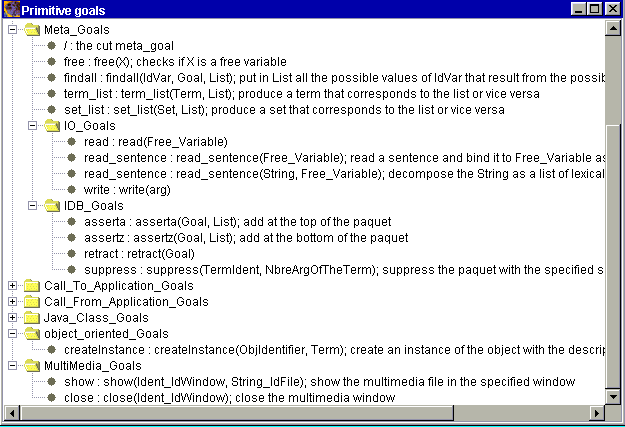
\includegraphics[scale=0.4]{EnvPrimHierMeta.png}
\end{center}
\caption{\label{EnvPrimHierMeta}Meta-Goals of PROLOG+CG}
\end{figure}

\end{latexonly}

\begin{htmlonly}

\begin{figure}
\begin{center}
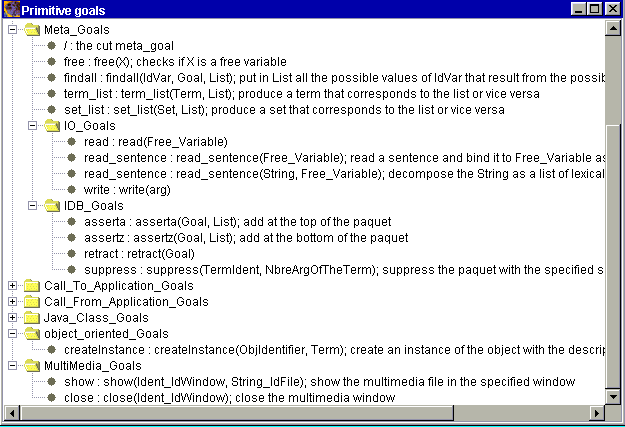
\includegraphics{EnvPrimHierMeta.png}
\end{center}
\caption{\label{EnvPrimHierMeta}Meta-Goals of PROLOG+CG}
\end{figure}

\end{htmlonly}


\subsection{Operator Cut/0 : ``/''}

To control the resolution process and to get a more efficient search
engine, PROLOG+CG, like most other Prolog versions, provides the cut
operator (represented often by ``\texttt{/}'' or
``\texttt{!}''). The cut operator ``\texttt{/}'' is considered
as a term with a special identifier (``\texttt{/}'') and no
arguments. It can be used as a goal in the tail of an inference rule.

\subsubsection{Example}

\begin{verbatim}
OurMember(e, (e | _)) :- /.
OurMember(e, (_ | x)) :- OurMember(e, x), /.

?- OurMember(x, (1, 3, 5, 7)).

{x = 1}
\end{verbatim}



\subsection{Operator free/1}

{\bf free(Variable)}

Checks if the variable is free.  Succeeds if it is, fails if it isn't.

\subsubsection{Example}


\begin{verbatim}
?- free(x).

{}

?- eq(x, 45), free(x).

no.
\end{verbatim}



\subsection{Operator findall/3}

{\bf findall(Variable, Goal, List)}

Return in List all the values of Variable that result from all the
possible resolutions of Goal

\subsubsection{Example}

\begin{verbatim}
donnee(4, jjj).
donnee(5, hhh).
donnee(6, kkkk).

data(10, kkk).
data(20, ddd).
data(30, ffff).
data(40, rrrr).

datum(x) :-
    donnee(x, _).
datum(x) :-
    data(x, _).

ex(m) :-   
    findall(a, datum(a), L),
    moyenne(L, m), /.

moyenne(L, m) :-
    length(L, n),
    somme(L, 0, s),
    val(m, div(s, n)), /.

somme((x|L), s1, s2) :-
    val(s3, add(x, s1)),
    somme(L, s3, s2), /.
    somme((), s, s).
\end{verbatim}

And to query:


\begin{verbatim}
?-ex(m).

{m = 16.428571428571427}
\end{verbatim}



\subsection{Operator read}

{\bf read(Free\_Variable)}

The argument of ``\texttt{read}'' should be a free variable at the
moment of its execution. When a read operation is executed, the system
will prompt the user with the symbol ``\texttt{|:}'' and the user
should give his data which could take several lines (a simple data
like a number, a boolean, an identifier, a string or a composed data
like a term, a list or a CG) and it should terminate with a point
``\texttt{.}''. Once his data is edited, the user should end with a
period (``\texttt{.}'') and press the key ``\texttt{Enter}''.

\subsubsection{Example}


\begin{verbatim}
?- read(x).
|: papa(Ahmed, Goerge).

{x = papa(Ahmed, Goerge)}
\end{verbatim}


\subsection{Operator read\_sentence/1}

{\bf read\_sentence(Free\_Variable)}

read\_sentence/1 reads a sentence (i.e. a sequence of characters) and
returns the list of ``\texttt{words}'' that composes it.  The sentence
should be endede with a period (``\texttt{.}''), which will be the
last ``\texttt{word}''.

You {\bf cannot} use \texttt{read\_sentence} from within a Java
applet.


\subsubsection{Example}


\begin{verbatim}
?- read_sentence(p).
|: this is a simple sentence, with a comma inside.

{p = ("this", "is", "a", "simple", "sentence", ",", "with", "a", 
 "comma", "inside", ".")}
\end{verbatim}



\subsection{Operator read\_sentence/2}

{\bf read\_sentence(Sentence, Free\_Variable)}

read\_sentence/2 returns in its second argument the list of words
that compose its first argument (which is a String).

You cannot use read\_sentence/2 from within a Java
applet.


\subsubsection{Example}


\begin{verbatim}
?- read_sentence("this is another sentence", L).

{L = ("this", "is", "another", "sentence")}
\end{verbatim}




\subsection{Operator write}

{\bf write(Data)}

The argument of write/1 is any PROLOG+CG data. A newline is not
added after the data has been written.  Strings and variables
containing strings will get their "double quotes" stripped.  write/1
always succeeds.


\subsection{writenl}

{\bf writenl(Data)}

The argument of writenl is any PROLOG+CG data. A newline IS added
after the data has been written.  Strings and variables containing
strings will get their "double quotes" stripped.  Writenl/2 always
succeeds.


\subsection{nl}
{\bf nl}

nl/0 takes no arguments, and prints a newline to the console either in
the normal Prolog+CG application GUI or in the Prolog+CG applet.  It
always succeeds.


\subsection{clearConsole}

{\bf clearConsole}

clearConsole/0 takes no arguments, and clears the console either in
the normal Prolog+CG application GUI or in the Prolog+CG applet.  It
always succeeds.


\subsection{asserta and assertz}

{\bf asserta(Goal,List\_Of\_Goals), assertz(Goal,List\_Of\_Goals)}

Asserta adds to the current program a new rule at the top of the
packet (if it exists) while assertz adds the rule at the bottom of the
packet. The first argument of asserta (and assertz) represents the
head of the new rule while the second argument represents the tail
expressed as a list. Of course, when the new rule is a fact, the list
is empty.

\subsection{retract/suppress}

{\bf retract(Goal) \& suppress(TermId, NumberOfArguments)}

Retract eliminates from the current program any rule with a head
that can be unified with its argument.

Suppress eliminates a whole packet of rules. The two arguments of
suppress (an identifier and an integer) enables the identification of
the packet.

\subsection{term\_list}

{\bf term\_list(Term, List)}

term\_list transforms a term to a list and vice versa.

\subsubsection{Example}


\begin{verbatim}
?- eq(x, papa), term_list(t, (x, Ahmed, y)).

{x = papa, t = papa(Ahmed, y), y = FREE}
\end{verbatim}



Now, suppose that we have a program that contains this packet:


\begin{verbatim}
papa(Ahmed, Soumia).
papa(Sahir, Fatine).
papa(Ahmed, Khalid).
\end{verbatim}


We ask again the previous question but in
addition, we want to execute the new composed term t:


\begin{verbatim}
?- eq(x, papa), term_list(t, (x, Ahmed, y)), t.

{x = papa, t = papa(Ahmed, Soumia), y = Soumia}
{x = papa, t = papa(Ahmed, Khalid), y = Khalid}
\end{verbatim}


\subsection{set\_list}

{\bf set\_list(Set, List)}

\texttt{set\_list} transforms a set to a list and vice versa.

\subsubsection{Example}


\begin{verbatim}
?- set_list(s, (Karim, Ahmed, Hicham)).

{s = {Karim, Ahmed, Hicham}}

?- set_list({Karim, Ahmed, Hicham}, L).

{L = (Karim, Ahmed, Hicham)}
\end{verbatim}


\section{The visual debugger of PROLOG+CG}\label{Sec:Debugger}

PROLOG+CG provides a powerful debugger that visualizes the inference
or resolution process as a construction or deconstruction (due to a
backtrack) of the inference tree. Figure \ref{Debug} gives a snapshot
that shows the debugger in action.  The figure shows also an auxiliary
window: ``a variable inspection window''. This type of window is
introduced next.


\begin{latexonly}

\begin{figure}
\begin{center}
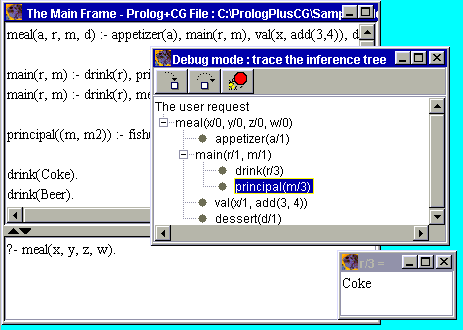
\includegraphics[scale=0.6]{Debug.png}
\end{center}
\caption{\label{Debug}The visual Debugger of PROLOG+CG}
\end{figure}

\end{latexonly}

\begin{htmlonly}

\begin{figure}
\begin{center}
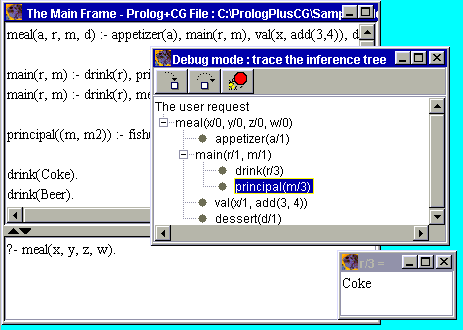
\includegraphics{Debug.png}
\end{center}
\caption{\label{Debug}The visual Debugger of PROLOG+CG}
\end{figure}

\end{htmlonly}



To debug (or trace, follow) the resolution/satisfaction of a request
(we assume that the program has been compiled), choose from the menu
the option ``\texttt{Build/Debug}'' and then activate the interpreter
as usual. The debug window appears. The current goal is the selected
node in the visual tree. Next, you must guide the debugger. Three main
actions are provided for that (they are represented by the three icons
in the toolBar of the debug window):

\begin{itemize}

\item {\bf ``\texttt{Inside}''} iconified by

\includegraphics{InStepBt.png}: ``\texttt{Inside the current step}''
means debug the current goal. If the fact is a fact, a message will
annonce it, otherwise the debugger will expand the visual tree and the
new current goal is the first ``\texttt{child}'' of the list. If the
current goal can't be resolved and the resolution process backtracks,
the debugger will backtrack also to the previous node.

\item {\bf ``\texttt{Skip}''} iconified by

\includegraphics{SkipStepBt.png}: ``\texttt{Skip}'' means not debug
the current goal. Again, if the current goal can't be resolved and the
resolution process backtracks, the debugger will backtrack also to the
previous node.

\item 

{\bf ``\texttt{Stop}''} iconified by 
\includegraphics{StopStepBt.png}:
Stop the debugger; the resolution process will continue without his
compagnon !

\end{itemize}

\subsection{Visualization of backtracking} 

The normal resolution process expands the inference tree; the
debugger will expand also the visual tree.  A backtrack step done by
the resolution process involves contraction and backward move in the
visual tree. Also, once the resolution process finds one solution and
writes it in the console panel, it will continue (by default) to
search for other solutions and the user can continue to use the
debugger to follow it.

\subsection{Goal/Variable inspection facility}

While debugging, it is very usefull to inspect the instanciation
form of a goal and/or the value of a specific variable (if the user
wants to do so). The visual debugger of PROLOG+CG allows the two:

\begin{itemize}

\item {\it {\bf inspect the instanciated form of a node:}} click on
the node (left-right, or right-left) to get the instanciated view of
the node. The content of the node is changed. You can click again to
come-back to the previous content of the node. So a sequence of
alternative left/right clicks will switch the content of the node from
the generic view to the instanciated one. You can also double-click to
get the instanciated view in an auxiliary window.

\item {\bf {\it inspect a specific variable:}} select from the main
menu the menu-item ``\texttt{Build|Inspect variable}'' , specify in
the text field the identifier of the variable (like ``\texttt{a/1}'' ,
without the double quotes) and press on ``\texttt{OK}''. An auxiliary
window will then appear with the value of the variable. An example of
such an auxiliary window is given in Figure \ref{Debug}.

\end{itemize}

\section{The Expert System Mode}\label{Sec:ES}

One of the main achievments of PROLOG was/is its use in the
development of expert system (ES) shells.  Most often, developers used
PROLOG to implement an ES shell, on top of it. In PROLOG+CG, the
kernel of an ES shell is integrated directly in the interpreter. Thus,
a simple check-item, as explained below, will switch the system from
the default resolution process to the ``ES shell resolution process''.

When the default resolution process (the usual interpreter of most
PROLOG versions) attempts to resolve a goal that is not a primitive
goal, neither a defined goal (no rule can be found so that its head
unifies with the goal), it will conclude that the goal can't be
resolved and it will backtrack.  However, the kernel of an ES shell
will proceed otherwise: it will not conclude that the goal can't be
resolved, it will ask the user about the truth of the goal
(``\texttt{is the current goal true or false ? : yes/no}''). The
process will conclude depending on the answer of the user and the user
answer will be added to the database, in order to be considered later
(and not to ask again and again the same question).

Actually, PROLOG+CG provides only this aspect of the ES shell. Other
aspects, like the explication of the resolution process behavior
(why/how) and forward chaining will be integrated in the next version
of PROLOG+CG.

To activate the ``expert system mode'' of PROLOG+CG, choose from the
main menu the action ``\texttt{Build/expert system mode}''. The
following examples illustrate this PROLOG+CG feature.

\subsection{Example 1: Propositional ES}

This example illustrates the possibility to define a {\it
propositional ES} using PROLOG+CG. A propositional ES is an ES where
any proposition is represented by a non-analyzable string. This later
is considered as a symbole (likewise in propositional logic, we use
symbols like p, q, r .. to represent propositions).


\begin{verbatim}
"animal is carnivore" :- "animal eats meat".
"animal is carnivore" :-
    "animal has pointed teeth",
    "animal has claws",
    "animal has forward eyes".

"animal is penguin" :-
    "animal is bird",
    "animal swims",
    "animal is black and white".

"animal is ungulate" :- "animal is mammal", "animal has hoofs".
"animal is ungulate" :- "animal is mammal", "animal chews cud".

"animal is mammal" :- "animal has hair".

"animal is ostrich" :- 
    "animal is bird", "animal has long neck",
    "animal has long legs", "animal is black and white".

"animal is zebra" :- 
    "animal is ungulate",  "animal has black stripes".

"animal is tiger" :-
    "animal is mammal",
    "animal is carnivore",
    "animal has twany color",
    "animal has black stripes".

"animal is cheetah" :-
    "animal is mammal",
    "animal is carnivore",
    "animal has twany color",
    "animal has dark spots".

"animal is giraffe" :-
    "animal is ungulate",
    "animal has long neck",
    "animal has long legs",
    "animal has dark spots".

"animal is bird" :- "animal has feathers".
"animal is bird" :- "animal flies", "animal lays eggs".
\end{verbatim}


To swith on the ``expert system mode'', the user has to choose from
the main menu the option ``\texttt{Build/Expert System Mode}''. Then,
compile the program. Here is a part of an interaction with the system.


\begin{verbatim}
?- "animal is tiger".
==> Is it true that: "animal has hair" ? tape y (for yes) or n
(for no) : y
==> Is it true that : "animal eats meat" ? tape y (for yes) or n
(for no) : y
==> Is it true that : "animal has twany color" ? tape y (for
yes) or n (for no) : y
==> Is it true that : "animal has black stripes" ? tape y (for
yes) or n (for no) : y
{}
==> Is it true that : "animal has pointed teeth" ? tape y (for
yes) or n (for no) : n
\end{verbatim}


After this interaction, PROLOG+CG added to
the program the following facts:


\begin{verbatim}
"animal has twany color".
"animal has black stripes".
"animal eats meat".
"animal has hair".
"animal has pointed teeth" :- fail.
\end{verbatim}

Note how the ``no'' answer is interpreted : assertion of a new rule
with the proposition as the head and the primitive goal
``\texttt{fail}'' as a tail. The {\bf fail} goal is no-satisfied by
definition.

The reformulation of this ES using predicates or terms instead of
non-analyzable String, is left as an exercice.

\subsection{Example 2: An ES that uses CG}

To illustrate the use of CG in the formulation of ES, we will
reformulate the same ES with the of CG only.


\begin{verbatim}
Universal > Object, Animal,
Person, Action, State, Attribute.
Object > Hair, Meat, Teeth, Claw, Eye.
Animal > Mammal, Carnivore, Cheetah.
Person > Man.
Action > Eat.
State > Belong.
Attribute > Color, Component, Twany, Dark, Pointed, Forward.

Man = Robert.
Animal = Yala.

[Animal : x]-is->[Cheetah] :-
    [Animal : x]-is->[Mammal],
    [Animal : x]-is->[Carnivore],
    [Animal : x]-colorOf->[Color]-attr->[Twany],
    [Animal : x]-partOf->[Component]-attr->[Dark].

[Animal : x]-is->[Mammal] :-
    [Animal : x]-poss->[Hair].


[Animal : x]-is->[Carnivore] :-
    [Animal : x]<-agnt-[Eat]-obj->[Meat].

[Animal : x]-is->[Carnivore] :-
    [Animal : x]-poss->[Teeth]-attr->[Pointed],
    [Animal : x]-poss->[Claw],
    [Animal : x]-has->[Eye]-attr->[Forward].
\end{verbatim}


Unlike the first formulation of the ES, we add to the CG formulation
the following fact, to give a ``\texttt{punch}'' to our example !



\begin{verbatim}
[Animal : Yala]-
        <-pat-[Belong]-bnfcre->[Man : Robert],
        -colorOf->[Color]-attr->[Twany],
        -poss->[Teeth]-attr->[Pointed],
        -has->[Eye]-attr->[Forward].
\end{verbatim}


Now, we can ask the following question:


\begin{verbatim}
?- [Animal : Yala]-is->[Cheetah].
==> The goal : [Animal : Yala]-poss->[Hair] cannot be infered
from what is known, so
==> Is it true that : [Animal : Yala]-poss->[Hair] ? tape y
(for yes) or n (for no) : y
==> The goal : [Eat] -
-obj->[Meat],
-agnt->[Animal : Yala] cannot be infered from what is known,
so
==> Is it true that : [Eat] -
-obj->[Meat],
-agnt->[Animal : Yala] ? tape y (for yes) or n (for no) : y
==> The goal : [Animal :
Yala]-partOf->[Component]-attr->[Dark] cannot be infered from
what is known, so
==> Is it true that : [Animal :
Yala]-partOf->[Component]-attr->[Dark] ? tape y (for yes) or
n (for no) : y
{}
==> The goal : [Animal : Yala]-poss->[Claw] cannot be infered
from what is known, so
==> Is it true that : [Animal : Yala]-poss->[Claw] ? tape y
(for yes) or n (for no) : n
\end{verbatim}



After this interaction, PROLOG+CG added to the program the following
facts:


\begin{verbatim}
[Animal : Yala]-poss->[Hair].
[Eat] -
    -obj->[Meat],
    -agnt->[Animal : Yala].
[Animal : Yala]-partOf->[Component]-attr->[Dark].
[Animal : Yala]-poss->[Claw] :- fail.
\end{verbatim}


\subsubsection{Remarks}

\begin{enumerate}

\item There is an important difference between the treatment of
``propositional'' or ``predicate'' ES and ``CG'' ES. For a predicate
ES, if the current goal or proposition to satisfy has the same
signature (the predicate identifier with the number of arguments) as
the head of a rule in the ES then we will not ask the user for the
truth of the goal/proposition, even if the goal is not satisfied. The
reason is that we have at least a rule that is able to compute the
truth of the goal/proposition. Concerning CG ES, we have not the
equivalent of a predicate signature : To satisfy a goal/proposition,
we have to consider all the rules with CG as head, if no one can be
unified with the goal, then we conclude that no existant rule can
infer the truth of the goal and so we ask the user for. Of course, if
the head can be unified, then we will not ask the reader, even if the
tail of the rule cannot be satisfied.

\item To return to the default mode of PROLOG+CG, don't forget to
switch off the ``Expert System Mode'' from the main menu and from
``\texttt{Build}''.

\end{enumerate}

\chapter{Object-Orientation}


\section{Objects, messages and OOP}\label{Sec:OO}

Sometime and especially for a big knowledge-base system (written in
Prolog), it is useful to partition the base in several partitions,
contexts or objects, each one includes a set of packets. Of course,
such a partition will be really useful only if the inference engine
(i.e., the resolution process) is adapted accordingly; resolution of a
goal will be restricted to the object where it is defined.  The
definition of objects and the contextual resolution of goals form the
basis for logic object-based programming.

\subsection{Objects in PROLOG+CG}

{\it An object} is a set of rules prefixed by terms with an
identical signature. An object has the following form:


\begin{verbatim}
T1::R1
T2::R2
...
Tn::Rn
\end{verbatim}


Where T1, T2, \ldots{}, Tn represent terms with the same signature and
R1, R2, \ldots{}, Rn stand for PROLOG+CG inference rules. The common
signature to the T1, T2, \ldots{}, Tn constitutes the {\it descriptor
of the object}.

Sending a message to an object will correspond to a contextual
resolution of a goal.

\subsubsection{Sending a message} 

{\it Sending a message} to an object is expressed as a {\it composed
goal}: T::G, where T represents a term and G a goal (i.e., which
could be a term, a CG or a variable). T::G can be read: ``send a
message to the object OT to execute (satisfy) the goal G''.  OT is the
object which its descriptor is the same as the signature of T.

To satisfy a composed goal T::G, the interpreter locates first an
object with a descriptor that corresponds to the signature of the term
T. Then it searches {\bf {\it inside}} the object for a prefixed rule
Ti::Ri such that T::G can be unified with Ti::HeadOf(Ri): the
interpreter tries to unify T with Ti and the goal G with the head of
the rule Ri.

\subsubsection{Remark} 

A rule can be prefixed also by a CG: {\bf CG::R}. In this case, all
the rules of the program that are prefixed by CG constitute one
object. Also, a composed goal can have the form : {\bf CG::Goal}.

\section{Samples IV}\label{Sec:SamplesIV}

This section presents two programs that illustrate the object-based
level of PROLOG+CG.

\subsection{Example 1}

(can be found in Samples/Others/Hamza.prlg):


\begin{verbatim}
Universal > PERSON, BIRTH, DATE.

hamza::[PERSON]-DateOfBirth->[BIRTH]-ptime->[DATE=(5,04,1995)].
hamza::Age(A) :-
    currentDate(D1), 
    hamza::[PERSON]-DateOfBirth->[BIRTH]-ptime->[DATE = D2],
    diffDate(D1, D2, A).

currentDate((14, 12, 1999)).

diffDate((x_Day2, y_month2, z_year2), 
         (x_Day1, y_month1, z_year1), 
         (x_Day, y_month, z_year)) :-
    val(x_Day, sub(x_Day2, x_Day1)), 
    val(y_month, sub(y_month2, y_month1)),
    val(z_year, sub(z_year2, z_year1)), /.
\end{verbatim}


Let us ask some questions:


\begin{verbatim}
?-  hamza::[BIRTH]-ptime->[DATE = d].
 
{d = (5, 4, 1995)}

?- hamza::Age(x).
 
{x = (9, 8, 4)}
\end{verbatim}



\subsection{Example 2}

(it can be found in Samples/Others/ConcStrs.prlg):


\begin{verbatim}
Universal > Animate, Inanimate, Action.
Action > Extract.
Animate > Person.
Person > Student, Employee.
Student > ResearchAssistant.
Employee > ResearchAssistant.
Inanimate > Text.
Text > Book.

// Conceptual structures for the type Extract 
// constitutes an object
Extract(canon)::[Extract]-
                     -agnt->[Person], 
                     -obj->[Inanimate].

Extract(schema)::[Extract]-
                    -agnt->[Person], 
                    -obj->[Text],
                    -target->[Book].

Extract(schema)::[Extract]-
                     -agnt->[Person], 
                     -obj->[Inanimate : *1],
                     -manr->[Strong],
                     -target->[Inanimate]-on->[Inanimate : *1].
\end{verbatim}


The next goal definition involves some comments: 

{\bf checkSchemas(v\_type)::G}: check if the given information in G
can be unified with a schema for the type v\_type. First, create a
term v\_term from the list (v\_type, schema), i.e. v\_type (schema),
v\_type will be replaced by its value. Second, search a schema
v\_schema for the type v\_type: v\_term::v\_schema. Third, check that
G can be unified with v\_schema.


\begin{verbatim}
checkSchemas(v_type)::G :-
       term_list(v_term, (v_type, schema)), 
       v_term::v_schema,
       eq(v_schema, G).
\end{verbatim}


Please note how the expressive power of PROLOG+CG allows for a very
abstract but ``effective'' formulation; search all the schema of a type
T so that they verify an information G. Note also how the message
({\bf v\_term::v\_schema}) is dynamically constructed;
constructed from two variables: the object descriptor is a variable
({\bf v\_term}) and the content of the message is a variable
({\bf v\_schema}).

Let us ask some questions:

{\it Get all the schemas of the type Extract:}

\begin{verbatim}
?- Extract(schema)::G.

{G = [Extract]-
              -agnt->[Person],
              -obj->[Text],
              -target->[Book]}
{G = [Extract]-
              -agnt->[Person],
              -obj->[Inanimate]<-on-[Inanimate : *1],
              -manr->[Strong],
              -target->[Inanimate : *1]}
\end{verbatim}


{\it Check if the given information ([Extract]-target->[Inanimate])
can be unified with one of the Extract schemas:}


\begin{verbatim}
?- checkSchemas(Extract)::[Extract]-target->[Inanimate].

{}
{}
\end{verbatim}



{\it And check for another information:}

\begin{verbatim}
?-checkSchemas(Extract)::[Inanimate]<-from-[Extract]-
                   ->obj->[Person].

no.
\end{verbatim}


\section{Inheritance rules and Object-oriented programming}\label{Sec:InheritanceAndOOP}

The object-oriented level of PROLOG+CG is
based on the approach proposed by McCabe [15]. Inheritance between
objects is defined by {\it inheritance rules}.

\subsection{Inheritance rule} 

It has the following form:

\begin{verbatim}
Term1 <- Term2
\end{verbatim}

where Term1 and Term2 are two terms that represent two objects. The
rule means: the object identified by Term1 is a specialization of the
object identified by Term2. If a message that is send to an object can
not be satisfied, the interpreter will search an inheritance rule for
that object (if it has) in order to delegate the message to its
super-object.

The next section gives an example that illustrates object-oriented
programming in PROLOG+CG.

\section{Samples V}\label{Sec:SamplesV}

The following example can be found in {\bf
Samples/Others/OORectSqre.prlg}. It illustrates how a class (as a set
of attributes and a set of methods) can be defined in PROLOG+CG. Let
us consider for instance the definition of the class
Rectangle. Rectangle is defined as an object (in the sense of
PROLOG+CG; an object in this language can represent a class like
Rectangle and/or a specific object like Hamza) identified by the term
{\bf Rectangle(H, W)}. Its static part (set of attributes) is
described by the first rule, represented by a CG. Notes that the
definition can have some semantic constraints, like the one expressed
in this example: the width should not be inferior to the height of the
rectangle. The constraints are formulated in the tail of the rule in
order to be evaluated when needed.

The two methods of Rectangle (Perimeter and Surface) are defined as
goals inside the object Rectangle(H, W).

Then, another class is defined: Square.  This class is defined as a
subclass of the class Rectangle. Notes the use of terms arguments to
precise the modality of such a relation between the two classes.


\begin{verbatim}
Universal > Form, Attribute.
Form > Rectangle.
Rectangle > Square.
Attribute > Perimeter, Surface, Width, Heigth, Beautiful.
 
Rectangle(H, W)::[Rectangle]-
                            -permOf->[Perimeter],
                            -surfOf->[Surface],
                            -widthOf->[Width = W],
                            -heigthOf->[Heigth = H] 
   :- not(inf(W, H)).

Rectangle(H, W)::Perimeter(P) :- 
   val(P, mul(2, add(H, W))).

Rectangle(H, W)::Surface(S) :-
   val(S, mul(H, W)).

// An inheritance rule.
Square(C) <- Rectangle(C, C).

Square(_)::[Square]-attr->[Beautiful].
\end{verbatim}



Let us consider some queries:


\begin{verbatim}
?- Rectangle(4,5)::G.
 
{G = [Rectangle] -
                 -permOf->[Perimeter],
                 -surfOf->[Surface],
                 -widthOf->[Width = 5],
                 -heigthOf->[Heigth = 4]}
{G = Perimeter(18)}
{G = Surface(20)}
\end{verbatim}


The next question illustrates the use of constraints. The question is:
is it possible to construct a rectangle with Width = 5 and Height = 4
? The answer to the question is no because the associated constraint
is not verified.


\begin{verbatim}
?- Rectangle(5,4)::[Width=5]<-widthOf-[Rectangle]-
                  ->heigthOf->[Heigth=4].
 
 no.
\end{verbatim}



Finally, the next request illustrates method inheritance:


\begin{verbatim}
?- Square(4)::Perimeter(P).
 
{P = 16}
\end{verbatim}



\section{The primitive goal createInstance}\label{Sec:CreateInstance}

PROLOG+CG provides the primitive goal {\bf createInstance(Ident,
Term)} which enables the creation of an instance Ident from an object
identified by Term.

When executed, {\bf createInstance(Ident, Term)} will add the
following inheritance rule to the program:

\begin{verbatim}
Ident <- Term.
\end{verbatim}

The following request illustrates the use
of createInstance (assuming the previous program of Rectangle and
Square):

\begin{verbatim}
?- createInstance(sq1, Square(6)), sq1::Surface(S).

{S = 36}
\end{verbatim}



\chapter{Prolog+CG and JAVA}

\section{Prolog+CG as a JAVA Applet}\label{Sec:JavaApplet}

\subsection{Introduction}

Prolog+CG can be embedded in an HTML page as a JAVA Applet.  This
section describes how to do so.

\subsection{What's provided?}

Basically, Prolog+CG as an applet has three GUI elements:

\begin{enumerate}

  \item A number of input text fields (from 0 to 5) where the end-user
  can write their input.

  \item A number of push buttons that can execute goals (from 1 to 5).

  \item A console area where the Prolog+CG program can communicate with
  the end-user.

\end{enumerate}

Figure \ref{PPCGAsJavaApplet} shows an example.

\begin{latexonly}

\begin{figure}
\begin{center}
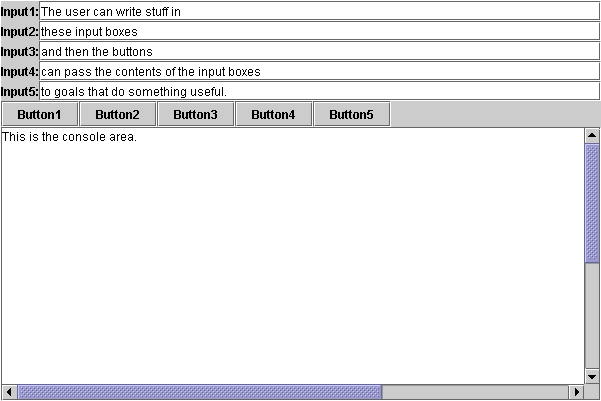
\includegraphics[scale=0.5]{PPCGAsJavaApplet.png}
\end{center}
\caption{\label{PPCGAsJavaApplet}PROLOG+CG as a Java applet}
\end{figure}

\end{latexonly}

\begin{htmlonly}

\begin{figure}
\begin{center}
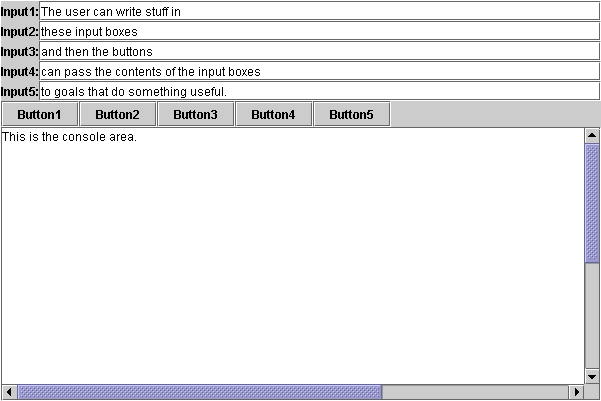
\includegraphics{PPCGAsJavaApplet.png}
\end{center}
\caption{\label{PPCGAsJavaApplet}PROLOG+CG as a Java applet}
\end{figure}

\end{htmlonly}




The console area can be written to with the usual write/1, writenl/1,
and nl/0 built-in primitives, and can be cleared with clearConsole/0.

Error messages from Prolog+CG are printed on the console.  However,
results from goals are not printed as in the normal Prolog+CG console
area.  Instead, the applet program is expected to communicate any
results to the user using the primitives just mentioned.

This design choice was made because the applet was envisaged as a
dialogue between a non-Prolog-programmer (a ``web user'') and the
Prolog+CG program.  Thus the applet is designed to be useful as a
demonstration of Prolog+CG for users who may not know Prolog.

The Prolog+CG program can use asserta/2 and assertz/2 and expect the
results to be remembered between the user's clicks on the buttons.

\subsection{Deploying an applet}

Once you have written your applet application as a Prolog+CG program,
go to ``\texttt{File|Deploy Applet}''.  If you haven't saved the
Prolog+CG program, you will be asked to do so.  Then a dialog will
appear, which looks like something like Figure \ref{AppletDeploymentDialog}:

\begin{latexonly}

\begin{figure}
\begin{center}
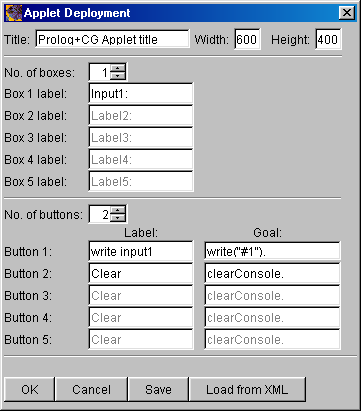
\includegraphics[scale=0.5]{AppletDeploymentDialog.png}
\end{center}
\caption{\label{AppletDeploymentDialog}Applet deployment dialog}
\end{figure}

\end{latexonly}

\begin{htmlonly}

\begin{figure}
\begin{center}
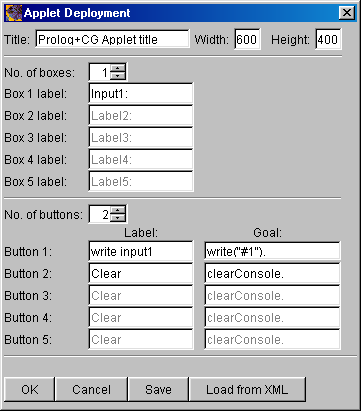
\includegraphics{AppletDeploymentDialog.png}
\end{center}
\caption{\label{AppletDeploymentDialog}Applet deployment dialog}
\end{figure}

\end{htmlonly}



You can define:

\begin{enumerate}

  \item The title of the applet.  This will appear as a <H1> title
  over the applet in the HTML that is written.  It will also appear in
  the <TITLE> tag in the header of the HTML.

  \item The width and the height.

  \item How many input boxes you want (from 0-5).

  \item The label next to each input box.

  \item How many buttons you want (from 1-5).

  \item The label of each button.

  \item The goal executed by each button.

\end{enumerate}

The four push-buttons at the bottom do the following:

\begin{itemize}

  \item {\bf OK:} Calls up the save procedure and, if the
  save procedure is successful, closes the dialog.

  \item {\bf Cancel:} Closes the dialog without saving.

  \item {\bf Save:} Calls up the save procedure.

  \item {\bf Load from XML:} Loads the dialog's parameters
  from an XML file previously saved by the dialog.

\end{itemize}

\subsubsection{What happens when you save?}

Well, a ``\texttt{Save}'' dialog box appears, which lets you choose a
directory (not a file) to which you can save the applet.

Once you have chosen the directory, the following four files will
be created in that directory:

\begin{itemize}

  \item {\bf index.html}: A simple HTML file containing a correctly
  formatted and filled \texttt{<APPLET>...</APPLET>} tag with all the
  necessary parameters.

  \item {\bf ppcgapplet.xml}: The applet parameters in XML,
  for easy loading with the ``\texttt{Load from XML}'' push-button.

  \item {\bf XXX.plgCG}: A copy of the Prolog+CG program
  which you had open when you called up the ``\texttt{Deploy Applet}'' dialog.
  This must be the Prolog+CG program which implements the application.

  \item {\bf PPCGApplet.jar}: The .jar file containing Prolog+CG and the implementation of the applet.

\end{itemize}

\subsubsection{Loading from XML}

Once you have saved an applet, its parameters will be saved in the XML
file ``\texttt{ppcgapplet.xml}''.  You can reload this at any point in
time by choosing the menu-item ``\texttt{File|Load Applet from XML}''.
If there is a program in memory, you will be asked to save it, since
it will be replaced by the applet's program.

You can also load an applet from XML from the ``\texttt{Deploy applet}''
dialog, by pressing the ``\texttt{Load from XML}'' button.

\subsubsection{Testing the applet}

To test the applet, open the ``\texttt{index.html}'' file in your webbrowser.
On Windows, this can be done by navigating to the directory where you
saved the applet and then opening ``\texttt{index.html}''.

\subsubsection{Copying to the webserver}

In order to fully deploy the applet, you must copy three of the
above four files to the webserver, namely all but the ppcgapplet.xml
file.  You can upload the ppcgapplet.xml file if you want to, but it
won't be used by the webserver.  Check with your webspace provider for
how to upload files.


\subsection{Writing an applet application}

\subsubsection{Introduction}

You can write your applet Prolog+CG program in the normal Prolog+CG
interface and test it there.  You will get results printed in the
console area as well as the output from your application, but the
results won't be printed when you run the program as an applet.

\subsubsection{The main key}

The key to writing the applet is to define from 1 to 5 goals that
serve as entry points into your application.  For example, you might
have a main/1 predicate that takes input from one of the input boxes.
This main/1 predicate then does something useful with the input, and
prints some results.  For example:


\begin{verbatim}
main(X) :- write("The input was: "), write(X), nl.
\end{verbatim}


\subsubsection{Binding buttons to goals}

Then you can bind one of the buttons to this goal.  For example, to
bind button 1 to call main with the contents of input-box 1, write the
following in the ``\texttt{goal}'' edit-box of the ``\texttt{Deploy
Applet}'' dialog box for Button 1:


\begin{verbatim}
main(#1).
\end{verbatim}


The \texttt{\#<number>} syntax works with \texttt{\#1}, \texttt{\#2},
\texttt{\#3}, \texttt{\#4}, and \texttt{\#5} to mean ``whatever is in
the input box with the same number at the time of pressing the
button.''

You can also write a predicate that takes two input-boxes:


\begin{verbatim}
main(X,Y) :- write("Input 1 is: '"), write(X), writenl("'."),
             write("Input 2 is: '"), write(X), writenl("'.").
\end{verbatim}


Then you can bind a button to input box 1 and input box 2 like this:


\begin{verbatim}
main(#1,#2).
\end{verbatim}


This syntax works to any number of times and in any order:


\begin{verbatim}
main(#1,#2,#3,#4,#5,#4,#3,#2,#1).
\end{verbatim}


If you wish to make a parameter into a string, do this:


\begin{verbatim}
main("#1").
\end{verbatim}


Please note that if the user then enters a "double quote" in input-box
1, Prolog+CG will give a syntax error.  This is because quotes are not
escaped before passing the contents of the input box.

\subsubsection{Help button}

It may be helpful for your end-users (the users of the applet) if you
include a button that says ``\texttt{Help}''.  This button can then
call a predicate which:

\begin{enumerate}

  \item Clears the console area with the clearConsole/0 built-in
  predicate.

  \item Writes a helpful help-message on what the applet does and how
  to use it, using a combination of write/1, writenl/1, and nl/0.

\end{enumerate}


\subsubsection{Clear}

It may also be helpful (but not always) if you add a button which
clears the console area using clearConsole/0.  This button could be
labelled ``\texttt{Clear}''.


\subsection{Writing the HTML yourself}

\subsubsection{Introduction}

The ``\texttt{File|Deploy Applet}'' procedure will write an HTML file
which works.  You can either take this file and customize it, or write
your own from scratch.  This section explains how.

\subsubsection{Applet Basics}

A JAVA Applet is defined by some HTML tags embedded in a larger HTML
file.  Specifically, the \texttt{<APPLET> ... </APPLET>} tag is
used. Inside the \texttt{<APPLET> ... <APPLET>} tag, the parameters to
the applet are given.

\subsubsection{APPLET-tag attributes}

The opening APPLET tag has some attributes, including the width, the
height, the name of the class file that implements the applet, and the
name of the .jar file that contains the applet class.  The
\texttt{<APPLET>} tag can look like this:


\begin{verbatim}
  <APPLET  code="PrologPlusCG/PrologPlusCGApplet.class"
    codebase="."
    archive="PPCGApplet.jar"
    width="600"
    height="400"
  >
\end{verbatim}


Of these, only the width and the height should be touched, unless you
know what you are doing.

\subsubsection{Applet parameters}

Inside the APPLET tag, one finds the parameters to the applet.  These
are given as single tags like this:


\begin{verbatim}
<PARAM name="parameter_name" value="parameter_value"  >
\end{verbatim}


The ``\texttt{paremeter\_name}'' must be replaced by one of the
parameter names in the table below, and the
``\texttt{parameter\_value}'' must be given as the desired value.

The parameters which the Prolog+CG applet understands are listed in Table \ref{AppletParameters}:


\begin{table}
\begin{tabular}{|l|l|l|l|}
\hline
  {\bf Name} &
  {\bf Type} &
  {\bf Comment} &
  {\bf Default value} \\ %%\tabularnewline  
\hline

  \parbox{2.0cm}{box1label\\
box2label\\
box3label\\
box4label\\
box5label} &
  String &
  \parbox{4.6cm}{The five labels of the five input boxes.} &
  \verb|""| \\ %%\tabularnewline 
\hline

  noofboxes &
  integer &
  \parbox{4.6cm}{The number of input boxes (values: 0-5).} &
  1 \\ %%\tabularnewline 
\hline

  noofbuttons &
  integer &
  \parbox{4.6cm}{The number of push-buttons (values: 1-5).} &
  1 \\ %%\tabularnewline 
\hline

  \parbox{2.0cm}{button1label\\
button2label\\
button3label\\
button4label\\
button5label} &
  String &
  \parbox{4.6cm}{The five labels of the five push-buttons.} &
  \texttt{"Clear"} \\ %%\tabularnewline 
\hline

  \parbox{2.0cm}{button1goal\\
button2goal\\
button3goal\\
button4goal\\
button5goal} &
  String & 
  \parbox{4.6cm}{The five goals of the five push-buttons.} &
  \texttt{"clearConsole."} \\ %%\tabularnewline 
\hline

  prologfile &
  String & 
  \parbox{4.6cm}{
  The name of the Prolog+CG program file as it appears on the webserver.} &
  \verb|""| \\ %%\tabularnewline 
\hline

  prologdir & 
  String &
  \parbox{4.6cm}{The name of the directory where the Prolog+CG program
  can be found, relative to the index.html file.  If you just leave
  this as \texttt{"."}, then the program can reside together with the
  HTML file.  If you make it empty or omit it, then \texttt{"."}
  will be used by default.} &
  \texttt{"."} \\ %%\tabularnewline 
\hline

\end{tabular}
\caption{\label{AppletParameters}Applet parameters}
\end{table}




\section{PROLOG+CG and JAVA}\label{Sec:PPCGAndJava}

(in collaboration with Prof. Dr. Bernard Moulin and his students:
Jeremi Gancet, David Nadeau and Olivier Rouleau, from Laval
university)

In the current version of Prolog+CG, PROLOG+CG can be activated from a
Java program and inversely, Java components (i.e. methods and
attributes of classes/objects) can be activated from a Prolog+CG
program. Figure \ref{EnvPrimHier4} gives the part of the primitive
goals hierarchy that concerns this side of PROLOG+CG.



\begin{latexonly}

\begin{figure}
\begin{center}
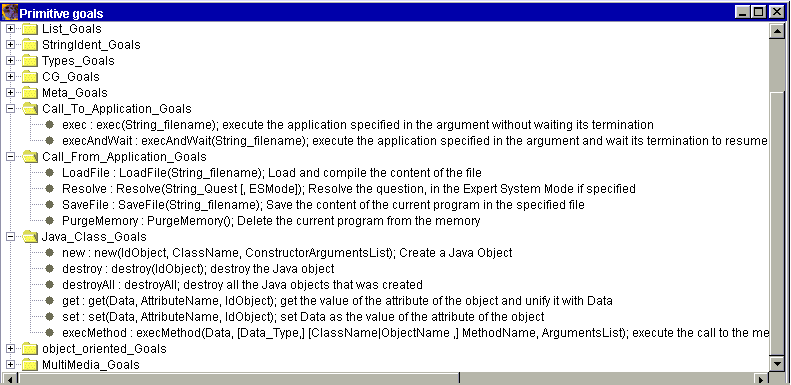
\includegraphics[scale=0.4]{EnvPrimHier4.png}
\end{center}
\caption{\label{EnvPrimHier4}Primitives of PROLOG+CG related to the
relation with JAVA}
\end{figure}

\end{latexonly}

\begin{htmlonly}

\begin{figure}
\begin{center}
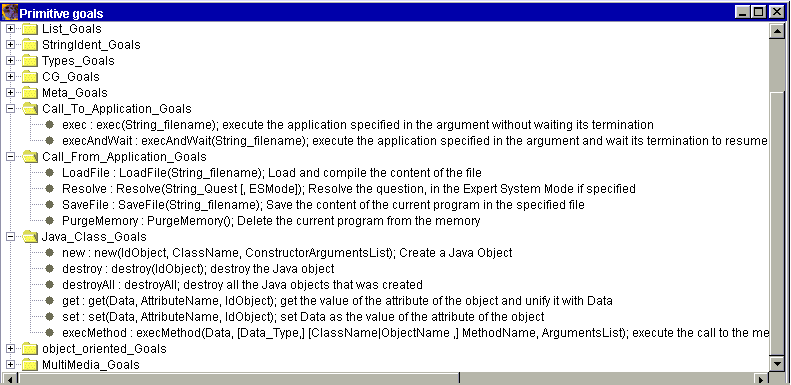
\includegraphics{EnvPrimHier4.png}
\end{center}
\caption{\label{EnvPrimHier4}Primitives of PROLOG+CG related to the
relation with JAVA}
\end{figure}

\end{htmlonly}



\subsection{Calling Prolog+CG from Java programs}

The Prolog language provides powerful reasoning
and symbolic manipulation capabilities, but it is not well suited
to implement the interface functionalities (windows, menus, link to
data bases, etc.) that object-oriented languages provide. Hence, a
good development strategy consists in using each Prolog+CG
programming paradigm to implement the functionalities that it best
supports. It is recommended to develop programs using Java and to
call the Prolog+CG modules when it is appropriate. This section
presents a set of primitives that Prolog+CG 2.0 provides in order
to call Prolog+CG modules from Java programs. The use of these
primitives is illustrated using a simple example.

{\bf Four primitives are used to exploit a Prolog+CG program
from a Java program}

\begin{itemize}

\item {\bf void LoadFile(String fileName)}

{\it ``\texttt{fileName}''} is the name of a Prolog+CG program. The role of
this primitive is to load a Prolog+CG program contained in the file
{\it ``\texttt{fileName}''.}

\item {\bf Vector Resolve(String Quest [, boolean ConvertResult]\newline
[, boolean ExpertSystemMode])}

the parameter {\it ``\texttt{Quest}''} is the request that Prolog+CG
should resolve. The optional parameter {\it
``\texttt{ConvertResult}''} specifies if the result should be
converted to string or not (it is set to true by default).  The
parameter {\it ``\texttt{ExpertSystemMode}'',} if it is specified, is
a boolean that indicates if Prolog+CG should behave like an expert
system shell or like a Prolog interpreter. This argument is set to
false by default. The primitive goal Resolve/3 returns all the
solutions in a Vector of hashtables; one solution being represented by
a hashtable. Since a solution is a set of couples <VariableIdentifier,
VariableValue>, it is natural to represent it as a hashtable with
VariableIdentifier as a key. To get the value of a variable in a
solution, one has to use the hashtable method ``\texttt{get(key)}''
where key stands for a variable identifier. Any value of a variable is
returned as a string (unless the parameter {\it
``\texttt{ConverseResult}''} is set to false). The examples below
illustrate this feature.

\item {\bf void SaveFile(String fileName)}

saves the current program in the Prolog+CG file
{\it ``\texttt{fileName}''.}

\item {\bf void PurgeMemory()}

deletes the current Prolog+CG program from memory.

\end{itemize}


\subsection{Example 1}

Assume that we have a Prolog+CG program
{\it ``\texttt{FamilyRelations.plgCG}''} which contains, among other things,
the following facts and rules:


\begin{verbatim}
[Man : John]-fatherOf->[Man : Peter].
[Woman : Deborah]-fatherOf->[Man : Peter].
[Man : John]-motherOf->[Woman : Clara].
[Person : x]-parentOf->[Man : y] :-
    [Person : x]-fatherOf->[Man : y].
[Person : x]-parentOf->[Woman : y] :-
    [Person : x]-motherOf->[Woman : y].
\end{verbatim}


From a Java program, we can assert new facts and
retract existing facts from the above Prolog+CG program and we can
ask questions and get answers.

Here is an example of such an interaction. The
Java file ``PrologPlusCG''
is implemented as a Java Package


\begin{verbatim}
import PrologPlusCG.PrologPlusCGFrame;
...
public void example() {
    ... any Java code
    // Load a Prolog+CG File
    LoadFile("FamilyRelations.plgCG");
    ... any Java code
    // Resolve a question
    Vector solutions = 
        Resolve("[Person : x]-parentOf->[Person : y]");
    // Make access to the solutions and to their content
    Hashtable solution;
    String valX, valY;
    For (Enumeration e = solutions.elements(); 
         e.hasMoreElements();) {
        // make access to a solution
        solution = (Hashtable) e.nextElement();
        // make access to the variable's value for the solution
        valX = (String) get("x");
        valY = (String) get("y");
        // make use of the variable's value
        ...
    };
    ...
    // assert a new fact in the Prolog+CG program
    Resolve("asserta([Man : Marc]-fatherOf->[Man : Clark], ())");
    ...
    // Save the current program in a new file
    SaveFile("FamilyRels1.plgCG");
    // Purge the current program from the memory
    PurgeMemory();
    ...
\end{verbatim}


\subsection{Example 2} 

{\it A simple syntactic analyzer}

\subsubsection{The Prolog+CG program file ``\texttt{AnalyseSynt.plgCG}''}


\begin{verbatim}
sentence(p, ph(_np, _vp)) :-
    read_sentence(p, L),
    np(L, L1, _np),
    vp(L1, (), _vp), /.

np((_det, _adj, _noun|L), L, np(det(_det), 
   adj(_adj), noun(_noun))) :-
    det(_art),
    adj(_adj),
    noun(_noun), /.

vp((_verb|L), L1, vp(verb(_verb), _np)) :-
    verb(_verb),
    np(L, L1, _np), /.


det("the").
det("a").
adj("beautiful").
noun("girl").
noun("apple").
verb("eat").
verb("eats").
\end{verbatim}


\subsubsection{The Java program}

File "FrmAnalyseSyntaxique.java"


\begin{verbatim}
import javax.swing.*;
import java.awt.*;
import java.util.*;
import java.awt.event.*;
import javax.swing.JTree.*;
import javax.swing.tree.*;
import PrologPlusCG.PrologPlusCGFrame;

public class FrmAnalyseSyntaxique extends JFrame {
  JTextArea jTextArea1 = new JTextArea();
  JScrollPane jspTextArea = new JScrollPane(jTextArea1);

  JButton BtAnalyse = new JButton();
  JButton BtNouvPhrase = new JButton();
  JButton BtFin = new JButton();

  JPanel jpnl = new JPanel();
  JTree jTree1;
  JScrollPane jspArbre;

  public static void main(String [] args) {
    FrmAnalyseSyntaxique unFrm = new FrmAnalyseSyntaxique();
  }

  public FrmAnalyseSyntaxique() {
    super();
    try {
      jbInit();
      this.show();
    }
    catch (Exception e) {
      e.printStackTrace();
    }
  }

  private void jbInit() throws Exception {
    setTitle("Analyse Syntaxique");
    getContentPane().setLayout(new BorderLayout());
    setSize(new Dimension(400, 500));

    jspTextArea.setMinimumSize(new Dimension(400,350));
    jspTextArea.setMaximumSize(new Dimension(400,350));
    jspTextArea.setBackground(SystemColor.info);
    jTextArea1.setText(" ");

    BtAnalyse.setLabel("Analyse");
    BtAnalyse.setPreferredSize(new Dimension(100,100));
    BtAnalyse.addActionListener(
           new java.awt.event.ActionListener() {
      public void actionPerformed(ActionEvent e) {
        BtAnalyse_actionPerformed(e);
      }
    });
    BtNouvPhrase.setLabel("Nouvelle Phrase");
    BtNouvPhrase.setPreferredSize(new Dimension(100,100));
    BtNouvPhrase.addActionListener(
              new java.awt.event.ActionListener() {
      public void actionPerformed(ActionEvent e) {
        BtNouvPhrase_actionPerformed(e);
      }
    });
    BtFin.setLabel("Fin");
    BtFin.setPreferredSize(new Dimension(100,100));
    BtFin.addActionListener(new java.awt.event.ActionListener() {
      public void actionPerformed(ActionEvent e) {
        BtFin_actionPerformed(e);
      }
    });

   jpnl.setPreferredSize(new Dimension(400, 350));
   jpnl.setBackground(SystemColor.info);

   getContentPane().add(jspTextArea, BorderLayout.NORTH);
   getContentPane().add(BtAnalyse, BorderLayout.WEST);
   getContentPane().add(BtNouvPhrase, BorderLayout.CENTER);
   getContentPane().add(BtFin, BorderLayout.EAST);
   getContentPane().add(jpnl, BorderLayout.SOUTH);
}

void BtAnalyse_actionPerformed(ActionEvent e) {
   PrologPlusCGFrame.LoadFile("AnalyseSynt.plgCG");
   Vector vect = PrologPlusCGFrame.Resolve("sentence(\""
                 + jTextArea1.getText() + "\", x).", false);
   // false in Resolve: indicates that the result shouldn't be 
   // converted to String
  if (vect == null)
    JOptionPane.showMessageDialog(this, 
           "The sentence is ungrammatical.", 
           "Warning", JOptionPane.OK_OPTION);
  else { // Draw the syntactic tree
    Hashtable solution = (Hashtable) vect.firstElement();
    getContentPane().remove(jpnl);
    jTree1 = new JTree((Vector) solution.get("x"));
    jspArbre = new JScrollPane(jTree1);
    getContentPane().add(jspArbre, BorderLayout.SOUTH);
    show();
  };
}

void BtNouvPhrase_actionPerformed(ActionEvent e) { 
  jTextArea1.setText(\verb|""|);
  try {
    this.getContentPane().remove(jspArbre);
    jspArbre.remove(jTree1);
    jTree1.removeAll();
    jTree1 = null;
    jspArbre = null;
    this.getContentPane().add(jpnl, BorderLayout.SOUTH);
  } catch(Exception ex) {};
  show();
}

void BtFin_actionPerformed(ActionEvent e) {
  System.exit(0);
  }
}
\end{verbatim}


Figure \ref{AppelAnalSynt} shows a snapshot of the directory and the
DOS console just before the execution of the above Java file.

\begin{latexonly}

\begin{figure}
\begin{center}
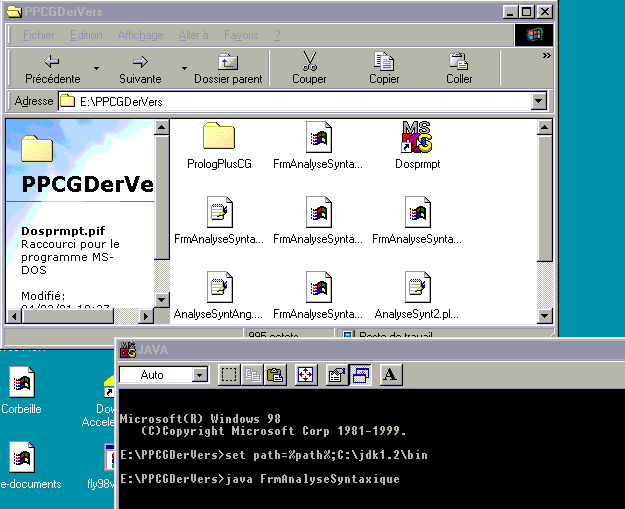
\includegraphics[scale=0.4]{AppelAnalSynt.png}
\end{center}
\caption{\label{AppelAnalSynt}Snapshot of the directory and the DOS
console just before the execution of the above Java file}
\end{figure}

\end{latexonly}

\begin{htmlonly}

\begin{figure}
\begin{center}
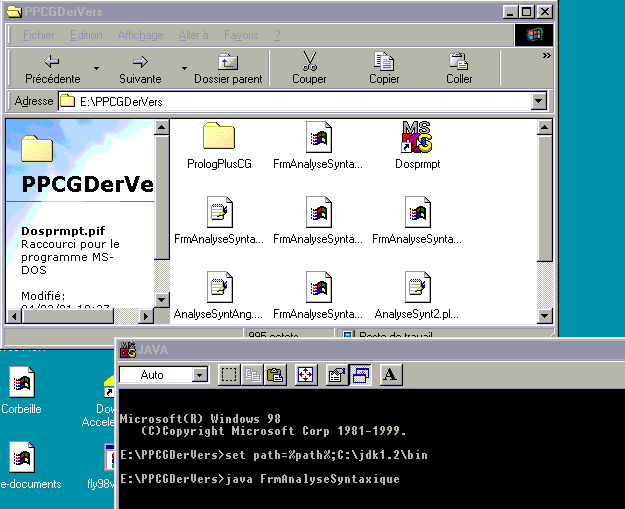
\includegraphics{AppelAnalSynt.png}
\end{center}
\caption{\label{AppelAnalSynt}Snapshot of the directory and the DOS
console just before the execution of the above Java file}
\end{figure}

\end{htmlonly}



Figure \ref{AnalySynt12} shows the result of the execution of the
above Java file.


\begin{latexonly}

\begin{figure}
\begin{center}
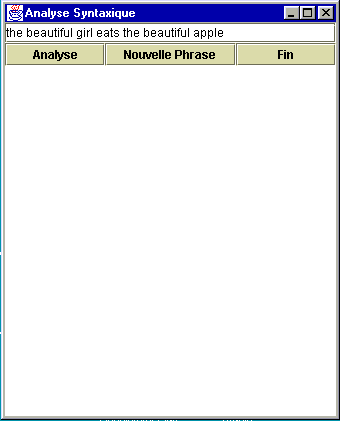
\includegraphics[scale=0.4]{AnalSynt1.png}
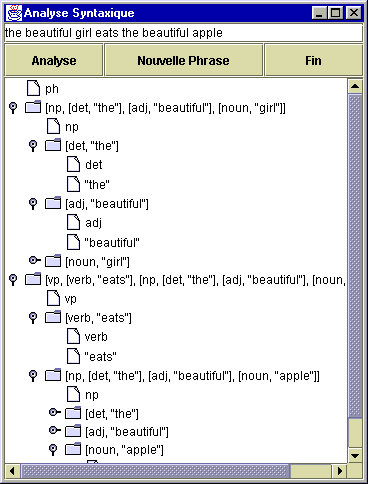
\includegraphics[scale=0.4]{AnalSynt2.png}
\end{center}
\caption{\label{AnalySynt12}(a) before the analysis~~~~~~~~~~~~~~(b)
after the analysis}
\end{figure}

\end{latexonly}

\begin{htmlonly}

\begin{figure}
\begin{center}
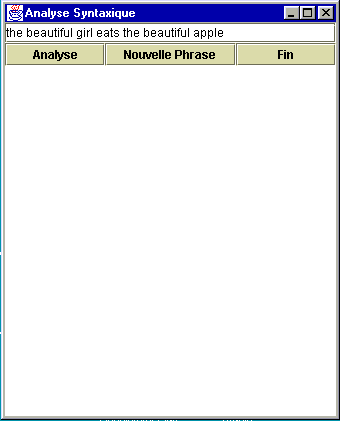
\includegraphics{AnalSynt1.png}
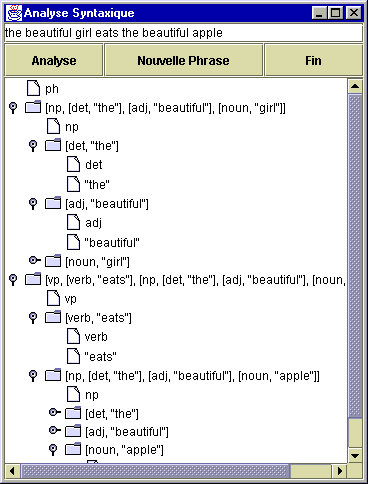
\includegraphics{AnalSynt2.png}
\end{center}
\caption{\label{AnalySynt12}(a) before the analysis~~~~~~~~~~~~~~(b)
after the analysis}
\end{figure}

\end{htmlonly}



The following four primitives are are ``{\em external}'' primitives of
Prolog+CG: ``\texttt{LoadFile}'', ``\texttt{Resolve}'',
``\texttt{SaveFile}'' and ``\texttt{PurgeMemory}''.  This means that
they are used in a Java Program to make use of a Prolog+CG
program. These simple external commands may look like details but they
are a tremendous step forward in making the Prolog+CG language a
concrete development tool. The interface inability to convey a sense
of usability and user-friendliness has long been a major obstacle in
using logic programs in real end-user developments.  For instance, it
is not unusual to have many lines of Prolog code to enter before
making a useful query. In addition, a lot of parameters in these lines
of code are very sensible to error and require that the user know the
program's internal workings fairly well to be able to get any valuable
information from the system. In addition, the answer has the typical
Prolog form (an output list) and it is sometimes very hard to
read. The output list (i.e. the solution) is neither sorted
alphabetically nor numerically. Finally, if the user wants additional
information on one of the listed items, an additional query is
necessary.

All these considerations find an elegant solution using the {\it
Java/Prolog+CG} interface. We have used this interface to develop a
simple Prolog+CG program (Figures \ref{Fig:InputScreen} and
\ref{Fig:OutputScreen}).  The front-end interface has been implemented
using Java and the reasoning part using Prolog+CG. The input screen
(Figure \ref{Fig:InputScreen}) offers lists and slider bars and
actually writes in the Prolog+CG program four assertions for the user,
using his selections. A results-screen (Figure \ref{Fig:OutputScreen})
then presents the output list which can be sorted using any
criteria. Additional information on a given list item can be obtained
with the simple press of a button (Figure \ref{Fig:OutputScreen}).

\begin{latexonly}

\begin{figure}
\begin{center}
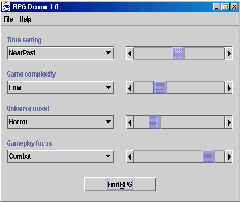
\includegraphics[scale=0.2]{Prolog1.jpg}
\end{center}
\caption{\label{Fig:InputScreen}Front-end interface for a Prolog+CG
program (Input screen)}
\end{figure}

\end{latexonly}

\begin{htmlonly}

\begin{figure}
\begin{center}
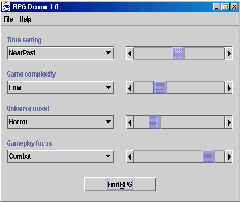
\includegraphics{Prolog1.jpg}
\end{center}
\caption{\label{Fig:InputScreen}Front-end interface for a Prolog+CG
program (Input screen)}
\end{figure}

\end{htmlonly}


\begin{latexonly}

\begin{figure}
\begin{center}
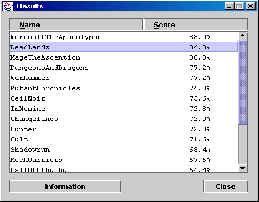
\includegraphics[scale=0.2]{Prolog2.jpg}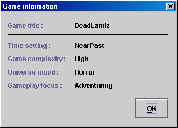
\includegraphics[scale=0.2]{Prolog3.jpg}
\end{center}
\caption{\label{Fig:OutputScreen}front-end interface for a Prolog+CG
program (Output screen)}
\end{figure}

\end{latexonly}

\begin{htmlonly}

\begin{figure}
\begin{center}
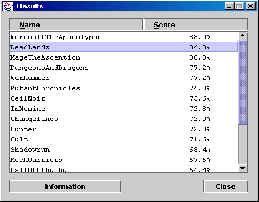
\includegraphics{Prolog2.jpg}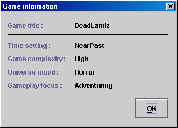
\includegraphics{Prolog3.jpg}
\end{center}
\caption{\label{Fig:OutputScreen}front-end interface for a Prolog+CG
program (Output screen)}
\end{figure}

\end{htmlonly}



Using this example, we wanted to emphasize the importance of having
interfaces between languages thus allowing each to be used for what it
is best at. This Prolog+CG functionality makes it a concrete
development tool easily usable in real projects. By allowing evolved
logic reasoning to be used in simple user-friendly applications as
well as complex Java code, the language moves beyond the traditional
academic boundaries.

\subsubsection{Note}

The The Expert System Mode of Prolog+CG can be exploited from a Java
program by using the primitives described in this Section. In this
case, the second argument of the primitive ``\texttt{Resolve/2}''
should be used and should be set to ``\texttt{true}''.



\subsection{Calling applications from a Prolog+CG program}

Prolog+CG 2.0 provides two primitives which allow calling an
executable application from a Prolog+CG program.  This is another way
to make use of Prolog+CG 's capabilities to work as a component of a
larger system.

\begin{itemize}

\item {\bf exec(ExecFileName):} starts the execution of the
application given by {\it ``\texttt{ExecFileName}''} and continues the
current resolution.

\item {\bf execAndWait(ExecFileName):} starts the execution of the
application {\it ``\texttt{ExecFileName}''} and waits for its
termination.  Then it resumes the current resolution of the Prolog+CG
program.

\end{itemize}

\subsubsection{Example}


\begin{verbatim}
ex1 :-
   eq(x, 45),
   exec("Synergy.exe"),
   writenl("Continue without waiting for the end of Synergy..."), 
   /.

ex2 :-
   eq(x, 45),
   execAndWait("Synergy.exe"),
   writenl("Continue after the end of Synergy ..."), /.
\end{verbatim}




The result of the execution of ex1 can be seen in Figure
\ref{Fig:ppcgsyn}.

\begin{latexonly}

\begin{figure}
\begin{center}
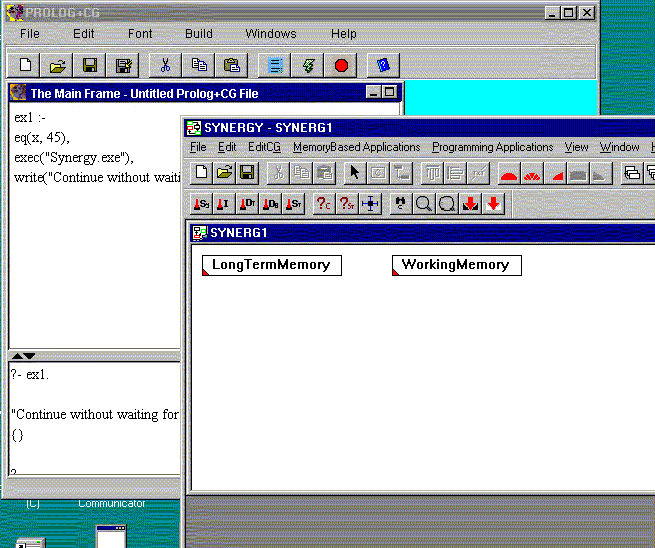
\includegraphics[scale=0.4]{ppcgsyn.png}
\end{center}
\caption{\label{Fig:ppcgsyn}Result of execution of ex1}
\end{figure}

\end{latexonly}

\begin{htmlonly}

\begin{figure}
\begin{center}
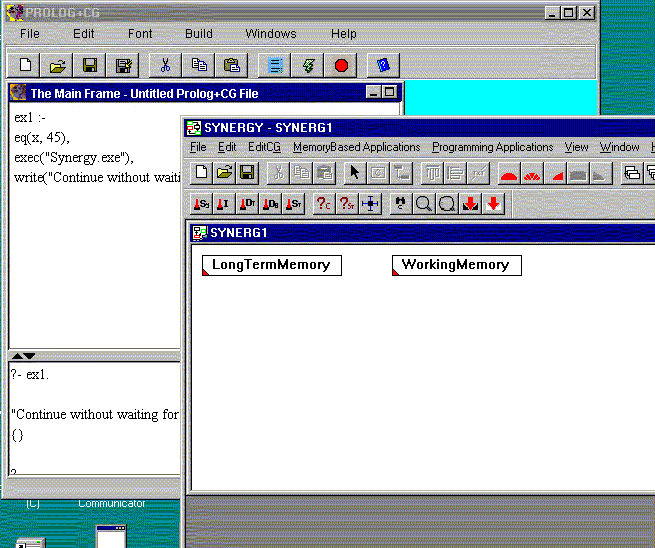
\includegraphics{ppcgsyn.png}
\end{center}
\caption{\label{Fig:ppcgsyn}Result of execution of ex1}
\end{figure}

\end{htmlonly}




\subsection{Using Java code from Prolog+CG}

Prolog+CG 2.0 provides several primitives allowing the use of Java
code and providing access to object-oriented capabilities. Indeed, new
Java objects can be created, used and destroyed from a Prolog+CG
program. These objects are considered as ``\texttt{global objects}'' of a
Prolog+CG program.

This section presents these primitives and briefly illustrates their
use.

\begin{itemize}

\item {\bf new(NewObjectIdent, JavaClass, ConstructorArguments):}
this primitive goal enables the creation of a new Java object. It
corresponds to the following Java instruction:

\begin{verbatim}
JavaClass NewObjectIdent = 
           new JavaClass(ConstructorArguments);
\end{verbatim}


\item {\bf destroy(ObjectIdent)}: this primitive goal destroys the
Java object identified by {\it ``\texttt{ObjectIdent}''}.

\item {\bf destroyAll}: this primitive goal destroys all the Java
objects that have been created in the current program.

\item {\bf get(Data, AttributeIdent, ObjectIdent)}: this primitive
goal can be used to get the value of the attribute {\it
``\texttt{AttributeIdent}''} of the object {\it
``\texttt{ObjectIdent}''.} The value is then unified with the first
argument {\it ``\texttt{Data}''.}

\item {\bf set(Data, AttributeIdent, ObjectIdent)}: this primitive
goal can be used to set {\it ``\texttt{Data}''} as the value of the
attribute {\it ``\texttt{AttributeIdent}''} of the object {\it
``\texttt{ObjectIdent}''.}

\item {\bf execMethod(Data\_Or\_void, JavaClass\_Or\_ObjectIdent,
MethodIdent, MethodArguments):} this primitive goal can be used to
call a method ``\texttt{MethodIdent}'', of a Java class (in the case
of a static method) or of a Java object
``\texttt{JavaClass\_Or\_ObjectIdent}'' with the argument list
``\texttt{MethodArguments}''. If the method is of type void then the
first argument of the primitive execMethod should be the keyword
``\texttt{void}''. Otherwise, the returned value is unified with the
first argument ``\texttt{Data\_Or\_void}''.

\item {\bf val(VariableIdent\_Or\_ObjectIdent, Expression\_Or\_ObjectIdent)
:} this primitive goal determines the value of its second
argument, which could be an expression or an object identifier. The
value of the expression (or the object) is then associated to the
variable (or to the object).

\end{itemize}

With calling Java code from Prolog+CG predicates
and calling Prolog+CG from Java code, the loop is closed and
the language offers both a powerful new representational
programming paradigm and an integrated way to access it
conveniently.

\subsubsection{Example 1} 

this simple example shows how an object (of a primitive or a
defined Java class) can be created and how the object methods can be
invoked.

\begin{verbatim}
explePPCGToJava(x,y) :-
    new(vct, "java.util.Vector", ()),
    execMethod(void, vct, "addElement", (4)),
    execMethod(void, vct, "addElement", (6)),
    execMethod(void, vct, "addElement", (10)),
    execMethod(void, vct, "addElement", (14)),
    execMethod(x, vct, "size", ()),
    execMethod(y, vct, "elementAt", (2)).
\end{verbatim}


And to use:


\begin{verbatim}
?- explePPCGToJava(x,y).

{x = 4, y = 10}

?-
\end{verbatim}

The next example shows the extendable feature of Prolog+CG. Suppose
for instance that someone needs a primitive to convert a string to an
integer. Instead of adding a new primitive to Prolog+CG to do that,
the user can use Java directly for that. It corresponds to a call to a
method of a class in Java that do such a job:



\begin{verbatim}
?- execMethod(c, "java.lang.Integer", "valueOf", ("345")), 
   sup(c, 300).

{c = 345}
\end{verbatim}


\subsubsection{Example 2}

{\it An application that calls Java code: SHRDLU-PCG} To
illustrate the expressive power of Prolog+CG and to show its
usefulness for the development of natural language processing
applications, we developed SHRDLU-PCG, a reformulation in Prolog+CG of
some aspects of the classic SHRDLU program [10]. In the Prolog+CG
program (see below), one can note the natural use of CG as a data
structure, beside term and list, and also the very use of variables in
CG: a variable can hold for a CG, a concept, a concept type, a
referent, a co-referent, a concept description (or value) and a
relation. This flexibility is very important from a programming
perspective.  SHRDLU-PCG also illustrates how Java classes (and their
attributes and methods) can be used from a Prolog+CG program.
SHRDLU-PCG simulates a very restricted natural language dialog between
a user and a robot that operates in a block-world. The robot can
create, move, push and pop 3D blocks. The robot is able to
``understand'' declarative, imperative and interrogative sentences and
to react accordingly. The 3D animation that results from such a dialog
is monitored thanks to the ``cooperation'' of the Prolog+CG program
SHRDLU-PCG with a Java3D program which provides the capability to
create a 3D canvas, to fill it with 3D objects (cube, cylinder,
sphere, pyramid) and to do some actions on them.

First, let us consider how the semantic analysis of a sentence and
especially the analysis of an imperative sentence is carried out.
Examples of imperative sentences are ``create a red pyramid
pyramid4.'', ``push the red pyramid on the big cube.'' and ``move the
blue sphere at the left of cube1.''.  As the components of the
sentence are analyzed, CGs that represent their semantic meaning are
constructed and then joined. This dynamic construction of CGs is in
itself an important feature of Prolog+CG.


 
\begin{verbatim}
// lexicon(Word, SyntacticCategory, TypeOrCGCanon)
lexicon("push", verb,[Push]-
     -obj->[Object],
     -on->[Object] ).
lexicon("create", verb,
[Create]-obj->[Object]-colorOf->[Color]).
Lexicon("sphere", noun, Sphere).

Verb(V, _CGCanon) :- lexicon(V, verb, _CGCanon).

// Syntax of imperative-sentence = Verb NP Complement.
// Complement = [Prep NP].
imperative_sentence((V|P1),
[Proposition: G]-mode->[Modality : imperative]) :-
    Verb(V, G_V),
    NP(P1, P2, E_NP1, S1),
    eq([T_Verb]-obj->E_N_G1, G_V),
    maximalJoin(G_V, E_N_G1, S1, E_NP1, G1_S1,_),
    complement(P2, T_Verb, G1_S1,G).
\end{verbatim}



\subsubsection{Comment on Verb/2} 

checks if V is a verb, if so, return the canon of the verb.

\subsubsection{Comment on imperative\_sentence/2}

imperative\_sentence(P, G) receives a sentence P, as a list of
words, and produces a CG G that represents its meaning. It starts by
recognizing the verb and then the noun phrase. The canon of the verb
(G\_V) is then joined with the CG corresponding to the noun phrase
(S1). This maximal join should satisfy however the following
constraint : the concept that represents the head of the noun phrase
has to be joined with the concept that represents the object of the
verb. So we have to locate these two concepts in the two CGs
respectively and then we have to consider them as ``entry concepts'' for
the maximal join in question; this later should start by the join of
the two entry concepts.  The entry concept for the CG G\_V that
represents the semantic meaning of the verb is located by the
following goal : 

       
\begin{verbatim}
eq([T_Verb]-obj->E_N_G1, G_V).
\end{verbatim}


To understand the effect of the above goal, let's consider this
request:

\begin{verbatim}
?- eq(G_V,[Create]-obj->[Sphere:sphere1]),
   eq([T_Verb]-obj->E_N_G1, G_V).

{G_V = [Create]-obj->[Sphere:sphere1], T_Verb = Create,E_N_G1 =
[Sphere:sphere1]}
\end{verbatim}


As a result of the above unification eq/2, the variable
``\texttt{E\_N\_G1}'' refers to the concept in ``\texttt{G\_V}'' that
represents the object of the verb. Note how the variable
``\texttt{T\_Verb}'' stands for the type of the concept and the
variable ``\texttt{E\_N\_G1}'' stands for the whole concept.  The
defined goal \texttt{NP/4} : \texttt{NP(P1, P2, E\_NP1, S1) } returns
the graph \texttt{S1} that represents the meaning of the noun phrase
as well as the entry concept \texttt{E\_NP1} in \texttt{S1}.

After the analysis of the verb and the noun phrase, the maximal join
of their semantic representations is done, producing a CG
\texttt{G1\_S1} and then, the semantic analysis of the complement is
initiated. If the complement is specified, its semantic representation
will be computed and then joined with the CG \texttt{G1\_S1}.

After the semantic analysis of an imperative sentence, the
``\texttt{robot}'' will consider its meaning as an order to be
executed. Hence and as a result of such an execution, the knowledge of
the ``\texttt{robot}'' will change (for instance, the position of an
object has to be modified) as well as the 3D animation that shows the
visual simulation of the robot behavior. The following Prolog+CG code
shows how all these aspects are related.


\begin{verbatim}
Shrdlu :-
    new(aShrdlu_Canvas3D, "PrologPlusCG.Shrdlu_Canvas3D", ()),
    read_sentence(_sentence),
    ShrdluDialog(_sentence), /.

ShrdluDialog(("end", ".")) :- /.
ShrdluDialog(_sentence) :-
    Semantic_Analysis(_sentence, _CG),   
    _CG,
    read_sentence(_s),
    ShrdluDialog(_s), /.
\end{verbatim}


\paragraph{Comment on the main goal Shrdlu:} this goal initiates the 3D
simulation as well as the restricted natural language dialog. In
particular, it specifies a call to the primitive goal ``\texttt{new}''
in order to create an instance of the defined Java 3D class
\texttt{Shrdlu\_Canvas3D}. Such a creation will involve, among other
actions, the display of a frame that contains a ``\texttt{robot}''
(Figure \ref{Fig:SHRDLU:ROBOT}).

\paragraph{Comment on the goal ShrdluDialog:} in the above definition of the goal ``\texttt{ShrdluDialog}'', note how the meaning of the sentence
(i.e. the CG ``\texttt{\_CG}'' that results from the semantic analysis
of ``\texttt{\_sentence}'') is put as a goal to be interpreted. Thus,
in the case of an imperative sentence, the goal-variable
``\texttt{\_CG}'' will be bound to the following CG :

[Proposition : G]-mode->[MODALITY : imperative]The proposition G (the
variable G will be bound to a CG) is interpreted as an order that
should be satisfied. Here is the Prolog+CG rule that naturally
formulates this interpretation :


\begin{verbatim}
[Proposition : G]-mode->[MODALITY : imperative] :-
    G.
\end{verbatim}



Each order is then executed according to its semantic
interpretation. For instance, the order to create an object with a
specific name and color is defined as follows : first assert the
existence of the object in the data base, then create a physical
object in the 3D canvas. Each kind of object (Cube, Sphere, Pyramid)
is created by a corresponding method in the defined Java class
``\texttt{Shrdlu\_Canvas3D}'' (Figure \ref{Fig:SHRDLU:CanvasClass}).


\begin{verbatim}
[Create]-obj->[T_Obj : _IdObj]-colorOf->[Color : C] :-
    asserta(object([T_Obj : _IdObj]-colorOf->[Color : C]), ()),
    execMethod(void, "PrologPlusCG.Shrdlu_Canvas3D", 
               T_Obj, (_IdObj, C)),
    /.

?- Shrdlu.
|:create the green sphere sphere1.
\end{verbatim}

\begin{latexonly}

\begin{figure}
\begin{center}
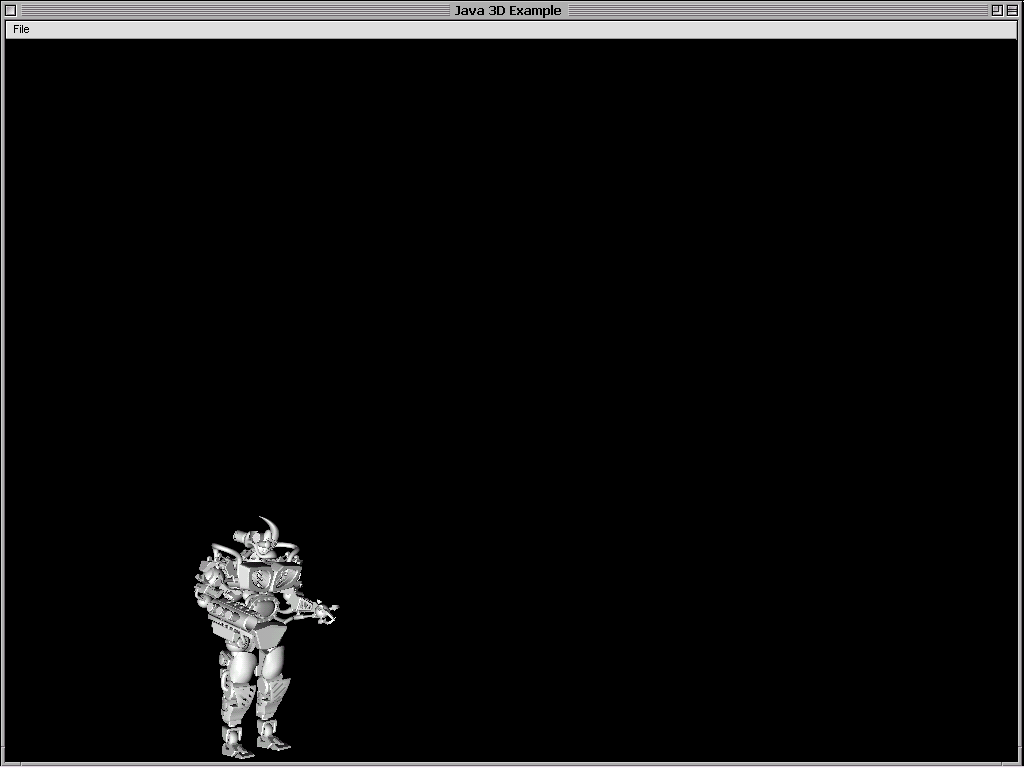
\includegraphics[scale=0.3]{Image1.png}
\end{center}
\caption{\label{Fig:SHRDLU:ROBOT}SHRDLU\_PCG in action}
\end{figure}

\end{latexonly}

\begin{htmlonly}

\begin{figure}
\begin{center}
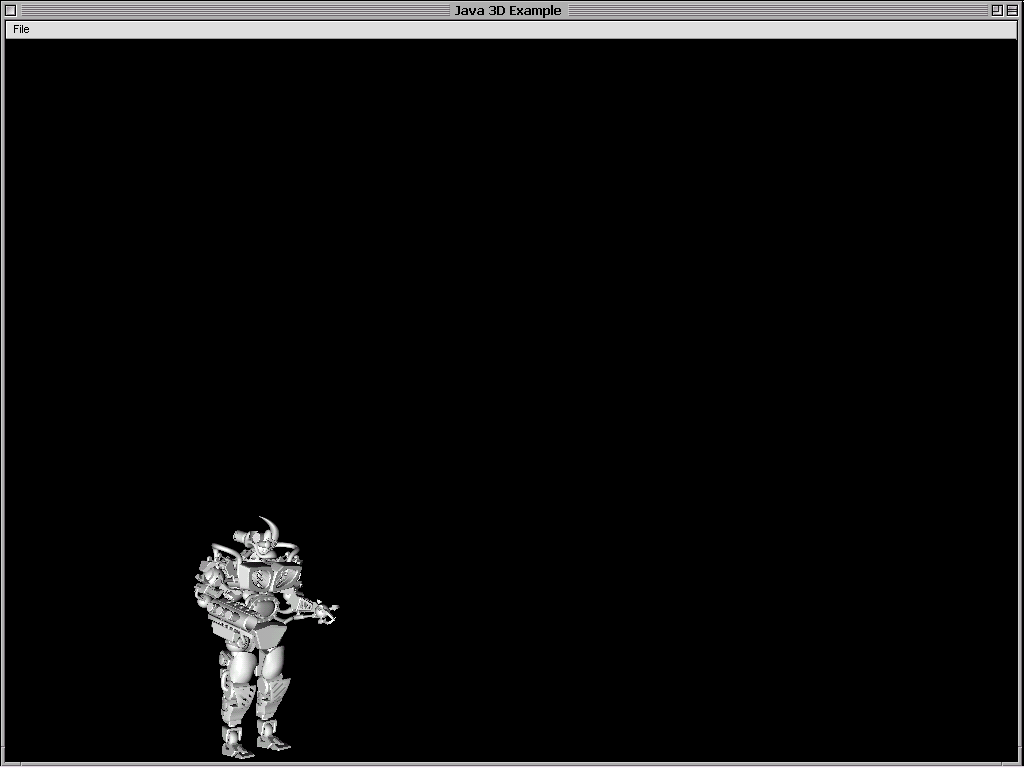
\includegraphics{Image1.png}
\end{center}
\caption{\label{Fig:SHRDLU:ROBOT}SHRDLU\_PCG in action}
\end{figure}

\end{htmlonly}


\begin{latexonly}

\begin{figure}
\begin{center}
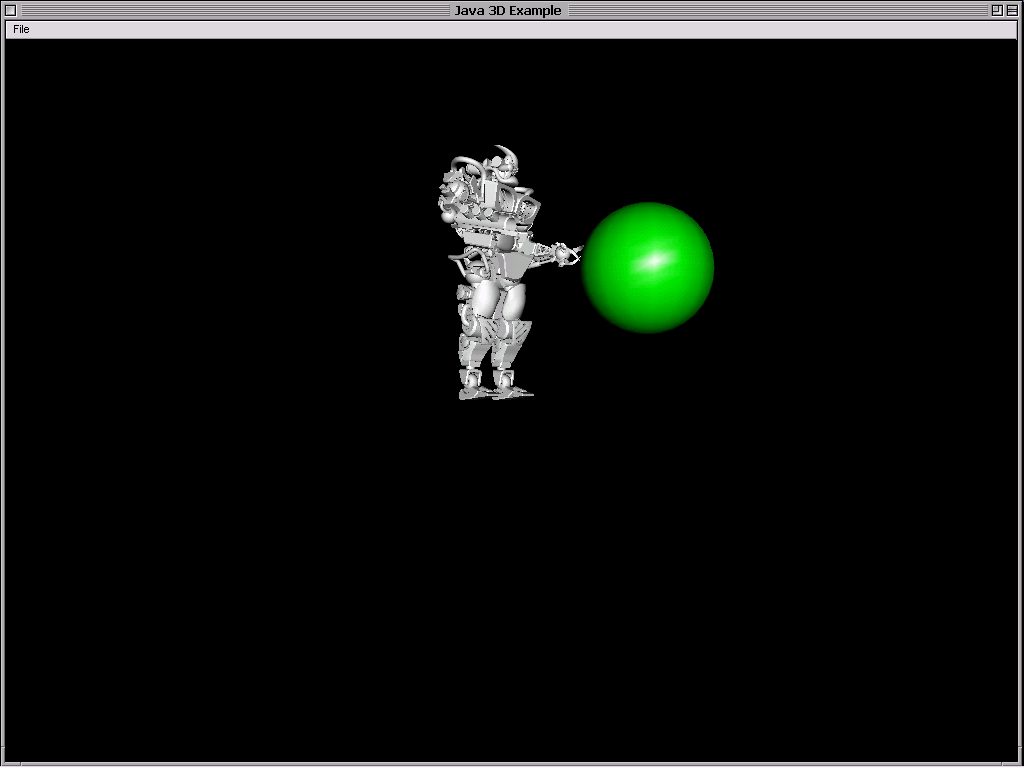
\includegraphics[scale=0.3]{Image2.png}
\end{center}
\caption{\label{Fig:SHRDLU:CanvasClass}SHRDLU\_PCG in action}
\end{figure}

\end{latexonly}

\begin{htmlonly}

\begin{figure}
\begin{center}
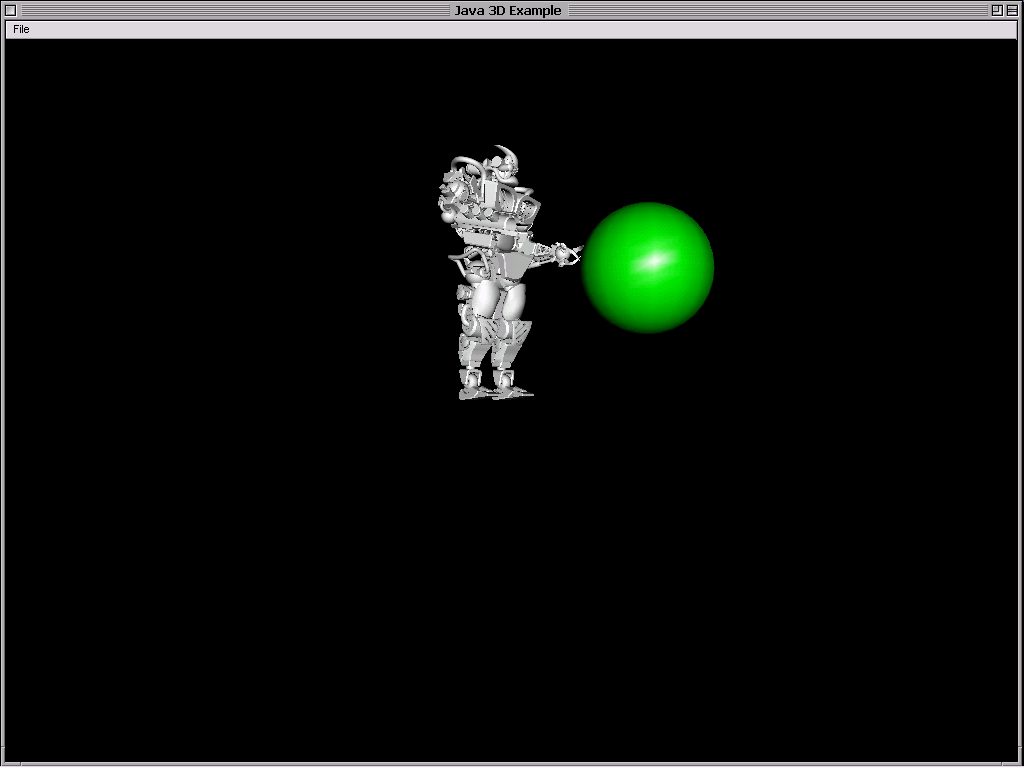
\includegraphics{Image2.png}
\end{center}
\caption{\label{Fig:SHRDLU:CanvasClass}SHRDLU\_PCG in action}
\end{figure}

\end{htmlonly}




\appendix

\chapter{The grammar of PROLOG+CG}\label{AppendixGrammar}


\begin{verbatim}
Prolog+CGProgram = (Rule | Comment) {(Rule | Comment)} .
Rule = Specialization_Rule | Instantiation_Rule 
     | Generalization_Rule | Inference_Rule .
Specialization_Rule = TypeIdentifier ">" TypeIdentifier
       {"," TypeIdentifier} "." .
Instantiation_Rule = TypeIdentifier "=" ReferentIdentifier
       {"," ReferentIdentifier} "." .
Generalization_Rule = ObjDescriptor "<-" ObjDescriptor "." .
Inference_Rule = Head [":-" Tail] "." .
Tail = Goal {"," Goal} .
Goal = SimpleGoal ["::" SimpleGoal] .
SimpleGoal = Term | CG | Variable .
Head = SimpleHead ["::" (SimpleHead | Variable)] .
SimpleHead = (Term | CG) .
ObjDescriptor = Term .
Term = Identifier [ "(" PrlgCGData {"," PrlgCGData} ")" ] .
List = "(" [ PrlgCGData {"," PrlgCGData} [ "|" Variable ] ] ")" .
PrlgCGData = Number | Boolean | Identifier | String
           | Variable | List | Term | CG .
CG = Concept [OutBranch | InBranch | Branches] .
Branches = "-" (OutBranch | InBranch) 
         {"," (OutBranch | InBranch) } [","] .
OutBranch = "-" RelationIdentifier "->" CG .
InBranch = "<-" RelationIdentifier "-" CG .
Concept = "[" Type [":" Referent] ["=" Value] "]" .
Type = TypeIdentifier | Variable .
Referent = ReferentIdentifier | Multi_Referent | Variable.
Value = PrlgCGData .
Comment = "//" {Character} .
TypeIdentifier = Identifier .
ReferentIdentifier = Identifier .
RelationIdentifier = Identifier .
Multi_Referent = "*" {Digit} .
Number = Digit { Digit } .
Boolean = "true" | "false" .
Identifier = Letter Letter { Letter | Digit | "_" } .
String = \verb|"""| { Letter | Digit | "_" } \verb|"""| .
Variable = ("_" { Letter | Digit | "_" }) | Letter 
         | (Letter (Digit | "_") { Letter | Digit | "_" } ) .
\end{verbatim}

\chapter{References}\label{Sec:References}
\begin{enumerate}
\item Ait-Kaci H. and R. Nasr. (1986), LOGIN : A logic programming
language with built-in inheritance, Journal Logic Programming, 3,
pp. 185-215.
\item Ait-Kaci H. and A. Podelski
(1992), Logic programming with functions over order-sorted feature
terms, in E. Lamma and P. Mello (Eds.), Extensions of Logic
Programming, Springer-Verlag, pp. 100-119.
\item Carpenter B. (1992), The logic
of typed feature structures, Cambridge Univ. Press.
\item Dichev C. (1993), Distributed
knowledge and data processing, in Proceeding of ICO'93
Montreal, Canada, pp. 279-282.
\item Dichev C. (1992), Logic
programming with worlds, in AI: Methodology, Systems,
Applications, North-Holland, pp. 57-67.
\item Fargues J., Landau M-C, Duguord
A. and Catach L. (1986), Conceptual Graphs for semantics and
knowledge processing, IBM Journal of Research and Development, vol.
30:1, pp. 70-79.
\item Fukunaga K. and S. Hirose
(1986), An experience with a Prolog-based object-oriented language,
in Proc. Of OOPSLA'86, pp. 224-231.
\item Garner B. J. and E. Tsui (1988),
General purpose inference engine for canonical graph models,
knowledge-Based Systems, 1:5, pp. 266-278.
\item Garner B. J., E. Tsui, D. Lui,
D. Lukose and J. Koh (1992), Extendible Graph Processing in
Knowledge Acquisition, Planning and Reasoning, in Nagle T. E., J.
A. Nagle, L. L. Gerholz and P. W. Eklund (Eds.), Conceptual
Structures: Current research and practice, Ellis
Horwood.
\item Herzog O. and C. --R.
Rollinger (Eds.) (1991), Text Understanding in LILOG,
Springer-Verlag.
\item Kabbaj A., C. Frasson, M.
Kaltenbach and J-Y Djamen (1994), A Conceptual and Contextual
Object-Oriented Logic Programming: The PROLOG++ language, in W. M.
Tepfenhart, J. P. Dick and J. F. Sowa (Eds.), Conceptual Structures
: Current Practices, ICCS'94, pp. 251-274.
\item Kabbaj A. (1996), Un systeme
multi-paradigme pour la manipulation des connaissances utilisant la
theorie des graphes conceptuels, Ph. D. Thesis, Univ. De Montreal,
Canada.
\item Kabbaj A. (1995),
Self-Organizing Knowledge Bases: The Integration Based Approach,
in the Proc. Of the Int. KRUSE Symposium: Knowledge Retrieval,
Use, and Storage for Efficiency, Santa Cruz, CA, USA, p.
64-68.
\item Kauffmann H. and A. Grumbach
(1986), MULTILOG: MULTIple worlds in LOGic programming, in the
proceeding of the 7th European Conference on
AI.
\item McCabe F. G. (1992), L\&O :
Logic and Objects, Prentice-Hall.
\item Monteiro L. and A. Porto (1989),
Contextual Logic Programming, in G. Levi and M. Martelli (Eds.),
Proc. 6th Int. Conf. And Symposium on Logic Programming,
MIT Press.
\item Moss C. (1994), Prolog++, The
Power of Object-Oriented and Logic Programming,
Addison-Wesley.
\item Pletat U. and K. von Luck
(1990), Knowledge Representation in LILOG, in Blasius and al.
(Eds.), Sorts and Types in Artificial Intelligence, LNAI
no. 418, Springer-Verlag.
\end{enumerate}
\end{document}
